
\documentclass[12pt]{report}
\usepackage{cuthesis}
\usepackage{amsmath}
\usepackage[font=small,format=plain,labelfont=bf,up,textfont=up]{caption}
\usepackage[T1]{fontenc}
\usepackage{graphicx}
\usepackage{subfigure}
\usepackage{float}
\usepackage{listings}
\usepackage{courier}
\usepackage[ruled,vlined]{algorithm2e}
\usepackage{verbatim}
\usepackage[toc, page]{appendix}
%\usepackage{natbib}
%\citestyle{nature}

\author{Guangfu Shi}
\title{Efficient Ray-Tracing Techniques Using GPU}
\degree{Master of Computer Science}
\dept{Computer Science}       % default is Comp.Sci.
\cosupervisor                   % if you also have a co-supervisor

%% New commands definitions
\newcommand{\myalgblankline} {\vspace{8pt}}
\newcommand{\mytriangle} {\(t\)}
\newcommand{\mytriangles} {\(T\)}
\newcommand{\mysplitplanes} {\(P\)}
\newcommand{\mysplitplanescan} {\(\hat{P}_{candidates}\)}
\newcommand{\mysplitplane} {\(p\)}
\newcommand{\mysplitplanek} {\(p_{k}\)}
\newcommand{\mysplitplanep} {\(p_{\xi}\)}
\newcommand{\mysplitplanea} {\(p_{0}\)}
\newcommand{\mysplitplaneb} {\(p_{1}\)}
\newcommand{\mysplitplanec} {\(p_{2}\)}
\newcommand{\mysplitplanen}[1] {\(p_#1\)}
\newcommand{\mybestsplitplane}                  {\(\hat{p}\)}
\newcommand{\mybestsplitplanek}                 {\(\hat{p}_{k}\)}
\newcommand{\mybestsplitplanep}                 {\(\hat{p}_{\xi}\)}
\newcommand{\mysplitplanepos} {\(\xi\)}
\newcommand{\myvoxel} {\(V\)}
\newcommand{\myaabb} {\(B\)}
\newcommand{\myaabbmin} {\(B_{min}\)}
\newcommand{\myaabbmax} {\(B_{max}\)} 
\newcommand{\myaabbmink} {\(B_{min,k}\)}
\newcommand{\myaabbmaxk} {\(B_{max,k}\)}
\newcommand{\myaabbside} {\(s\)}
\newcommand{\myleftchildbox} {\(V_{L}\)}
\newcommand{\myrightchildbox} {\(V_{R}\)}

\newcommand{\mynumtri} {\(N\)}
\newcommand{\mynumtrileft} {\(N_{L}\)}
\newcommand{\mynumtriright} {\(N_{R}\)}
\newcommand{\mynumtrileftk}[1] {\(N_{L,#1}\)}
\newcommand{\mynumtrirightk}[1] {\(N_{R,#1}\)}

\newcommand{\mykt} {\(K_{T}\)}
\newcommand{\myki} {\(K_{I}\)}
\newcommand{\mysapleft} {\(P_{L}\)}
\newcommand{\mysapright} {\(P_{R}\)}
\newcommand{\mysahcost} {\(C_{V}(p)\)} 
\newcommand{\mycostp} {\(C_{p}\)}
\newcommand{\mycostmin} {\(\hat{C}_{min}\)}
\newcommand{\mysahlambda} {\(\lambda(p)\)}
\newcommand{\mydimension} {k}
\newcommand{\myinfty} {\(\infty\)}
\newcommand{\myemptyset} {\(\emptyset\)}
\newcommand{\mytrilist} {\(T\)}
\newcommand{\mylefttrilist} {\(T_{L}\)}
\newcommand{\myrighttrilist} {\(T_{R}\)}
\newcommand{\mylefttrilistbest} {\(T_{l}\)}
\newcommand{\myrighttrilistbest} {\(T_{r}\)}
\newcommand{\mynumtrilist}[1] {\(\lvert\)#1\(\rvert\)}

% number of start, end triangles
\newcommand{\mynumtristartp}            {\(p^{+}\)}
\newcommand{\mynumtriendp}              {\(p^{-}\)}
\newcommand{\mynumtristartip}[1]        {\(p_{#1}^{+}\)}
\newcommand{\mynumtriendip}[1]          {\(p_{#1}^{-}\)}

% event data structure field, triangle, position and event type
\newcommand{\myevent}                   {\(e\)}
\newcommand{\myeventt}                  {\(e_{t}\)}
\newcommand{\myeventp}                  {\(e_{\xi}\)}
\newcommand{\myeventtype}               {\(e_{type}\)}
\newcommand{\myeventk}                  {\(e_{k}\)} 
\newcommand{\myeventlist}               {\(E\)}
\newcommand{\myeventlistleft}           {\(E_{L}\)}
\newcommand{\myeventlistright}          {\(E_{R}\)}
\newcommand{\myeventlistleftk}[1]       {\(E_{L}\)[#1]}
\newcommand{\myeventlistrightk}[1]      {\(E_{R}\)[#1]}
\newcommand{\myeventlistpi}[1]          {\(E_{p}\)[#1]}
\newcommand{\myeventlistppi}[1]         {\(E_{\xi}\)[#1]}
\newcommand{\myeventlistki}[1]          {\(E_{k}\)[#1]}
\newcommand{\myeventlistpki}[1]         {\(E_{p,k}\)[#1]}
\newcommand{\myeventlistti}[1]          {\(E_{type}[#1]\)}
\newcommand{\myeventlistk}[1]           {\(E_{#1}\)}
\newcommand{\mynumeventlist}            {\(E_{num}\)}
\newcommand{\myeventtypeend}            {\(-\)}
\newcommand{\myeventtypestart}          {\(+\)}

\newcommand{\mytriflagsarray}[1]        {\(flags\)[#1]} 
\newcommand{\mytriflagleft}             {\(LeftFlagBit\)}         
\newcommand{\mytriflagright}            {\(RightFlagBit\)}

\newcommand{\mynode}                    {\(n\)}
%\newcommnad{\mytrichuk}                 {\(k\)}


% Macros for algorithm complexity
\newcommand{\mycomplexityconst}         {\(O(1)\)}
\newcommand{\mycomplexityn}             {\(O(N)\)}
\newcommand{\mycomplexitysqrtn}         {\(O(N^2)\)}
\newcommand{\mycomplexitynlogn}         {\(O(N\log{N})\)}

% Macros for algorithms descriptions
\newcommand{\myfunc}                    {\textbf{function} }

% Useful Macros
\newcommand{\myopand}                   {\(\wedge\)}
\newcommand{\myopless}                  {\(<\)}
\newcommand{\myopgreater}               {\(>\)}
\newcommand{\myopin}                    {\(\in\)}

\newcommand{\mynaive}                   {na\"{\i}ve}
\newcommand{\myNaive}                   {Na\"{\i}ve}

% Source Code Formatting
\lstset{
         %basicstyle=\footnotesize\ttfamily, % Standardschrift
	 basicstyle=\small\ttfamily,
         %numbers=left,               % Ort der Zeilennummern
         numberstyle=\tiny,          % Stil der Zeilennummern
         %stepnumber=2,               % Abstand zwischen den Zeilennummern
         numbersep=5pt,              % Abstand der Nummern zum Text
         tabsize=2,                  % Groesse von Tabs
         extendedchars=true,         %
         breaklines=true,            % Zeilen werden Umgebrochen
         keywordstyle=\color{red},
	 %frame=t|b,         
 %        keywordstyle=[1]\textbf,    % Stil der Keywords
 %        keywordstyle=[2]\textbf,    %
 %        keywordstyle=[3]\textbf,    %
 %        keywordstyle=[4]\textbf,   \sqrt{\sqrt{}} %
         stringstyle=\color{white}\ttfamily, % Farbe der String
         showspaces=false,           % Leerzeichen anzeigen
         showtabs=false,             % Tabs anzeigen ?
         xleftmargin=17pt,
         framexleftmargin=17pt,
         framexrightmargin=5pt,
         framexbottommargin=4pt,
         %backgroundcolor=\color{lightgray},
         showstringspaces=false      % Leerzeichen in Strings anzeigen ? 
   	 captionpos=b
 } 


%---- Set figures path ----

% For Windows
%\graphicspath{{C:/Users/lenovo/thesis/working/thesis/graphics/}}

% For Mac
%\graphicspath{{/Users/steveca/thesis/working/thesis/graphics/}}

% For Linux 
\graphicspath{{/home/stevegocoding/thesis/working/thesis/graphics/}}

\begin{document}

\begin{abstract}
  Text of abstract.  
\end{abstract}

\begin{acknowledgments}
  Text of acknowledgments.
\end{acknowledgments}

%%%%%%%%%%%%%%%%%%%%%%%%%%%%%%%%%%%%%%%%%%%%%%%%%%%%%%%%%%%%%%%%%%%%%%%%%%%%%%%
%% Body of Thesis goes here.
%%%%%%%%%%%%%%%%%%%%%%%%%%%%%%%%%%%%%%%%%%%%%%%%%%%%%%%%%%%%%%%%%%%%%%%%%%%%%%%

% Set the page numbering style
\pagenumbering{arabic}
\setcounter{page}{1}

%------------------------
% Chapter 1 : Introduction

\chapter{Introduction}
Recently, with the dramatically boost of computational power of the current generati on CPU hardware, there has been a surge of new interetest in ray tracing as a core rendering algorithm for real-time applications such as video games since it is applicable to push the rendering task to interactive level on powerful computing devices which are easily accessible for a mainstream PC platform. Recently emerged powerful graphics processing units (GPUs) and flexible programming model provides researchers and developers with the ability to have the critical part of the algorithm parallelized and capture many secondary rendering effects such as shadows, refelections and refraction.


\paragraph{}
In the context of computer graphics, the term \emph{rendering} refers to the process of generating a two-dimension image from a three-dimensional virtual scene. Various rendering techniques have been widely used in many fields where computers are needed to generate images. Based on the algorithm used for the rendering process, rendering approach can be classified to two major categories: rasterization-based rendering and ray tracing-based rendering. 

\paragraph{}
At high level, rasterazation algorithm iterats projects the polygons, which forms the geometry objects in the scene, into screen space for rendering. With the application of Z-buffer, we could have a correct occlusion result, however, it may cause redundant raster and shading calculations which is also known \emph{overdraw}. One of the biggest advantages to a rasterization renderer is that a simple, immediate-mode graphics pipeline can be interfaced and only a set of geometry is required to be submitted to the renderer per frame without any need to introduce any acceleration structure (AS) of the scene. This pipeline interface could lead to a hardware implementation to this pipeline interface can be fast and able to handle the dynamic scene interactively. However, the weakness of rasterization rendering, which is its inablity to properly render secondary effects such as reflection, shadows and refraction, is vital especially in the fields where high quality rendering is required. It is required to adopt some multiple pass techniques to achieve such effects which are inefficient and produce visible artifacts. 

\paragraph{}
The idea behind ray tracing is straight-forward, instead of projecting geomery into screen, ray tracing shoots rays from the virtual camera into scene space and finds intersection points with the geometry object, and then secondary rays can be generated from the intersection point and cast into the scene for secondary effects. Once the intersection points are found, the final colours are going to be calculated and produce the final image. The major advantage of ray tracing over rasterization is its inherent correctness in presenting the optical phenomenon in the final image, no other special techniques need to be adopted to achieve shadows, reflection and refraction such secondary effects. Due to the nature of ray tracing, massive demand of computation power is the shortcoming and becomes the major barrier in the way to bring ray tracing to real-time applications.
 
\paragraph{}
The essential ray tracing task is to find the intersection points between rays and geometry, it is safe to classify ray tracing as a spatial searching problem, therefore, it will be helpful to incorporate a kind of AS which subdivides the scene to achieve efficient searching of intersection points. The AS, however, leads to a more complex hardware implementation since the rendering is no longer immediate and how to effiently build and maintain the AS bring more challenges on boosting the performance ray tracer. 

\paragraph{}
In addition to accelerate the ray tracing algorithmically, the revolutionary development of computing hardware driven by \emph{Moore's law} opens up another opportunity that cannot be ignored to make the ray tracing faster. Current generation x86 Central Processing Unit (CPU) is designed to maximize the parallelism including \emph{Instruction Level Parallelism} and \emph{Thread Level Parallelism}, these new features interest researchers to present new ideas and algorithms to take advantage of, such as rays packet traversal algorithm. Another common computing device in a system, which is the Graphics Processin Unit (GPU), has become much more powerful especially in float-point computing, furthermore, more flexible programming model and massive parralelism architecture make it as an alternetive device to use for ray tracing. However, none of these optimization approaches is automatically ann cheap, data structures and algorithms have to be carefully re-designed to be friendly to a specific device, and some constrains also have to be considered or they will significantly hit the overall performance. 

中文测试 latex

%------------------------

%-------------------------
% Chapter 2: Background

\chapter{Background}
\label{ch:background}
\setcounter{figure}{1}      % reset the figure counter

\section{Ray Tracing Algorithm Overview}

The ray-tracing algorithm is adopted by most photorealistic rendering system to generate a highly realistic image of a 3D scene. The core concept of the ray-tracing algorithm is straightforward, it is based on shooting the ray from the view point to a 3D scene as it interacts with the objects and light source in the scene. It can be understood as the reversed process of how our eyes perceive the world, which is receiving the light rays emitted by the light source and bounced off to the eyes. To simulates the physical phenomenon, a rendering system will have to model  the following key components : 

\begin{description} 	
	\item[Camera] \hfill \\
		The camera defines the position from where the scene is being observed and how the rays are generated. As an abstraction of the real camera, the camera in the rendering sytem is typically modeled with an eye position and the image or film in front of the eye, expecting the answer to what the color to display at each point in the image? Give the eye position as the origin and a point on the image, a ray can be generated by the camera and will be shot to the scene and the ray-object intersection test can be performed to determine the color value of that point on the image.  

	\item[Scene Description] \hfill \\ 
		The ``scene'' to be rendered is conceptually a database of ``geometric primitives'', which can be from simple geometric shapes such as polygons, spheres to complex shapes such as Bezier or NURBS patches. In fact, ray tracing can handle \emph{any} type of primitives as long as there is a proper algorithm to compute and intersection between ray and the primitive.

		Choosing the types of geometric primitive the ray tracer is going to support is an important design decision to make. The ray tracer can directly support complex primitives without tessellating them into polygon, thus they can be ray traced very efficiently and accurate, for example, directly compute the intersection between the ray and a sphere is almost trivial, while a tessellated sphere requires hundreds of triangles for a reasonable accuracy. However, the ray tracer that only supports these high-level primitives suffers from huge complexity and poor maintainability. Specific routine has to be implemented to support new type of primitive. On the other hand, supporting only triangles leads to a simple and optimized ray tracer implementation, the intersection calculation routine between a ray and triangle is quite efficient. Furthermore, triangle-based mesh can be used to approximate all of the high-level primitives very well and has a widely usage in the industrial application such as video games, CAD and movies. In conclusion, a triangle-based ray tracer is a more preferable design due to its simplicity and usability.

	\item[Ray Casting] \hfill \\
		Ray casting, the key problem for a ray-tracer to solve, is to shoot rays through each pixels on the image into the scene and then find out which geometric primitive, if any, that the ray hit first and where intersection point is. All the objects in the scene will be tested against the ray the first one will be selected. Given a ray \(r\) in parametric form:
		\begin{equation}
			r(t) = o + td
		\end{equation}
		where \( o \) is the ray's origin and \( d \) is the direction vector which is usually normalized so that the parameter \( t \) can be simply treated as the distance from the origin. The valid range of \( t \) is \( [0, \infty] \). With surface defined by an implicit function \( F(x, y, z) = 0 \), it is easy to find the intersection point by substituting the ray equation into the implicit equation to obtain a new function whose only parameter is \( t \), solving this function for \( t \), and substitute the smallest positive root into the ray equation to find the desired point. If there are no positive roots, the ray must miss the surface. The intersection point is not sufficient, ray-tracer also needs to know the additional properties of the surface such as normal vector and materials at that point to perform the shading stage later.

		As most scenes contains multiple objects, the brute-force approach that test the ray against each object can be too inefficient. To improve the performance, the acceleration structure is adopted by the ray-tracers to quickly cull whole groups of objects during the ray intersection process. The acceleration structures will be discussed in more detail in the following section.

		\begin{figure}[hpt]
			\centering
			\subfigure[]{ 
			\label{fig:RayCastingA}	%% label for first subfigure 
			\fbox{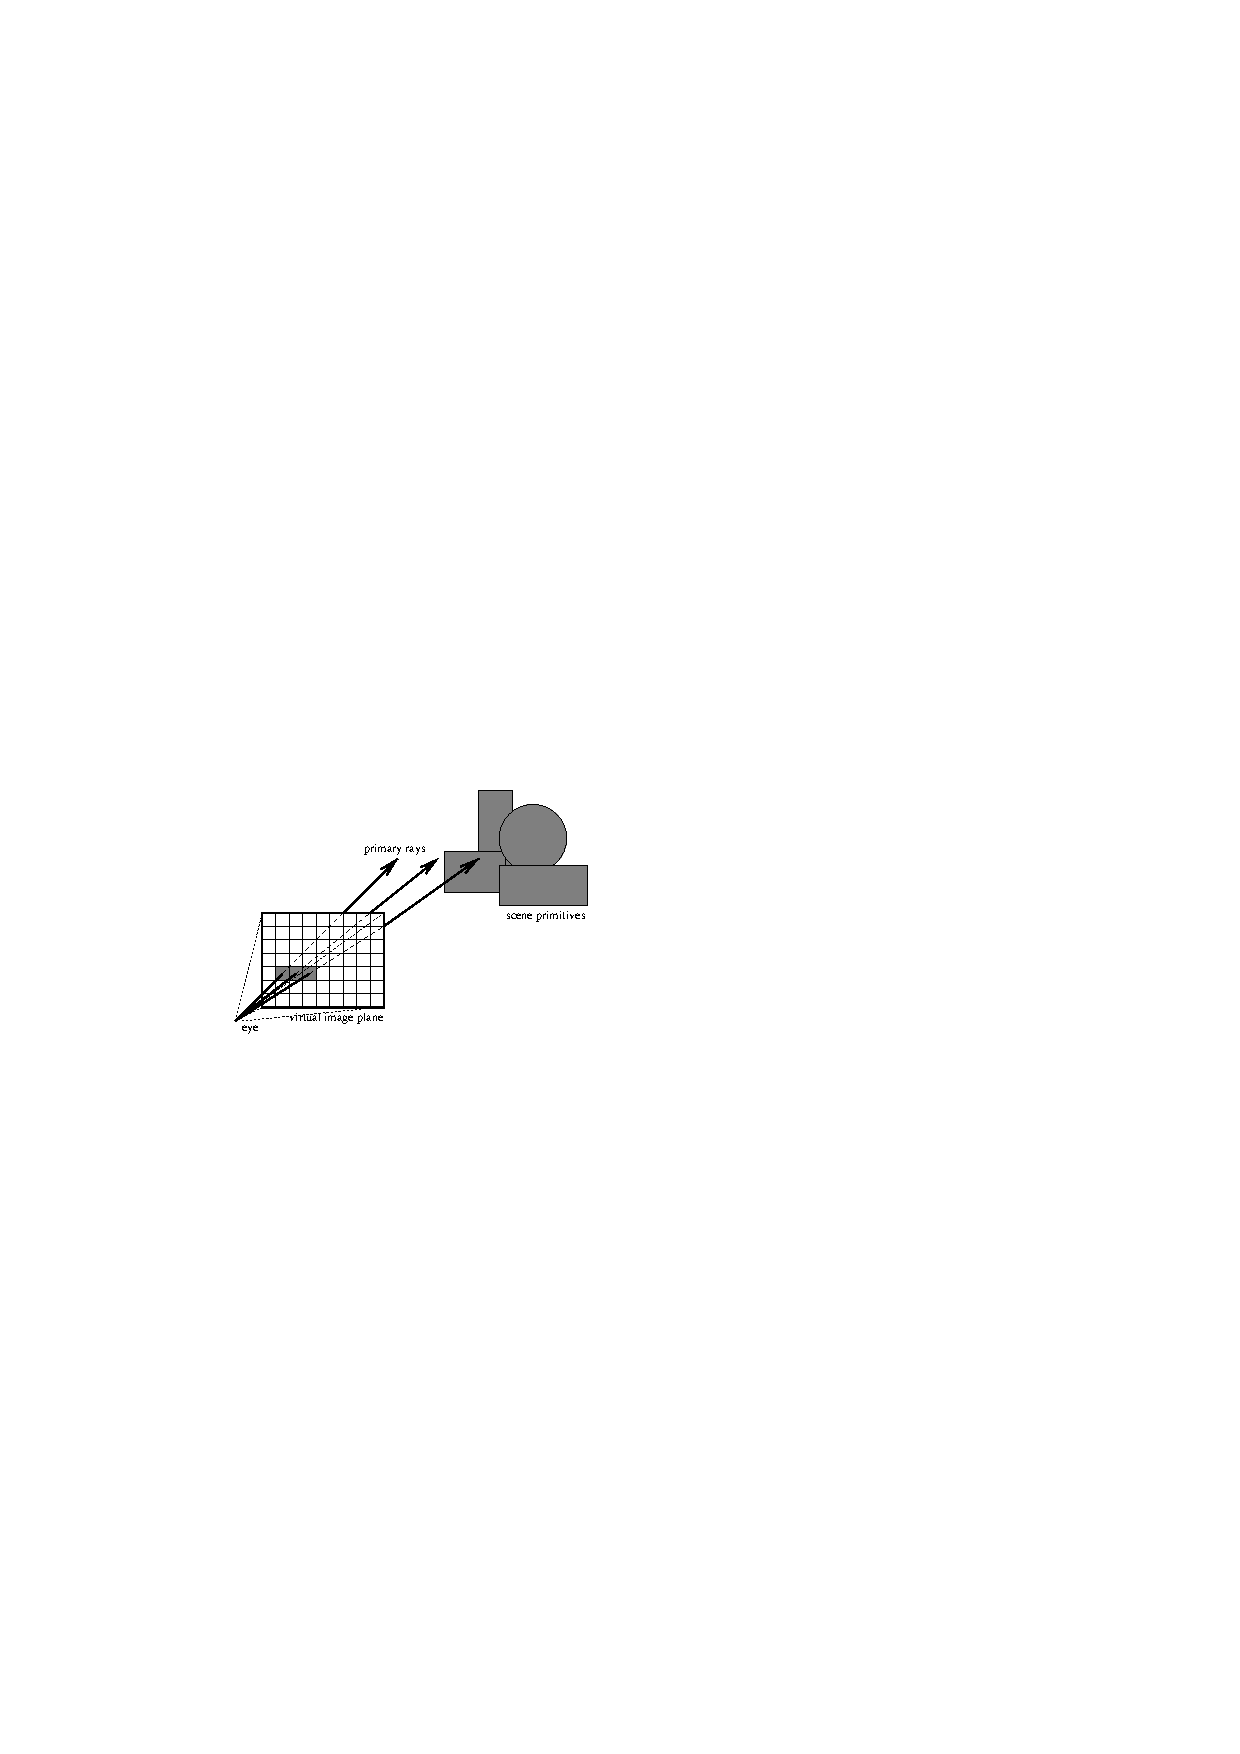
\includegraphics[width=0.42\linewidth]{figRayCastA.pdf}}}
			\hspace{0.01in} 
			\subfigure[]{
			\label{fig:RayCastingB}	%% label for second subfigure
			\fbox{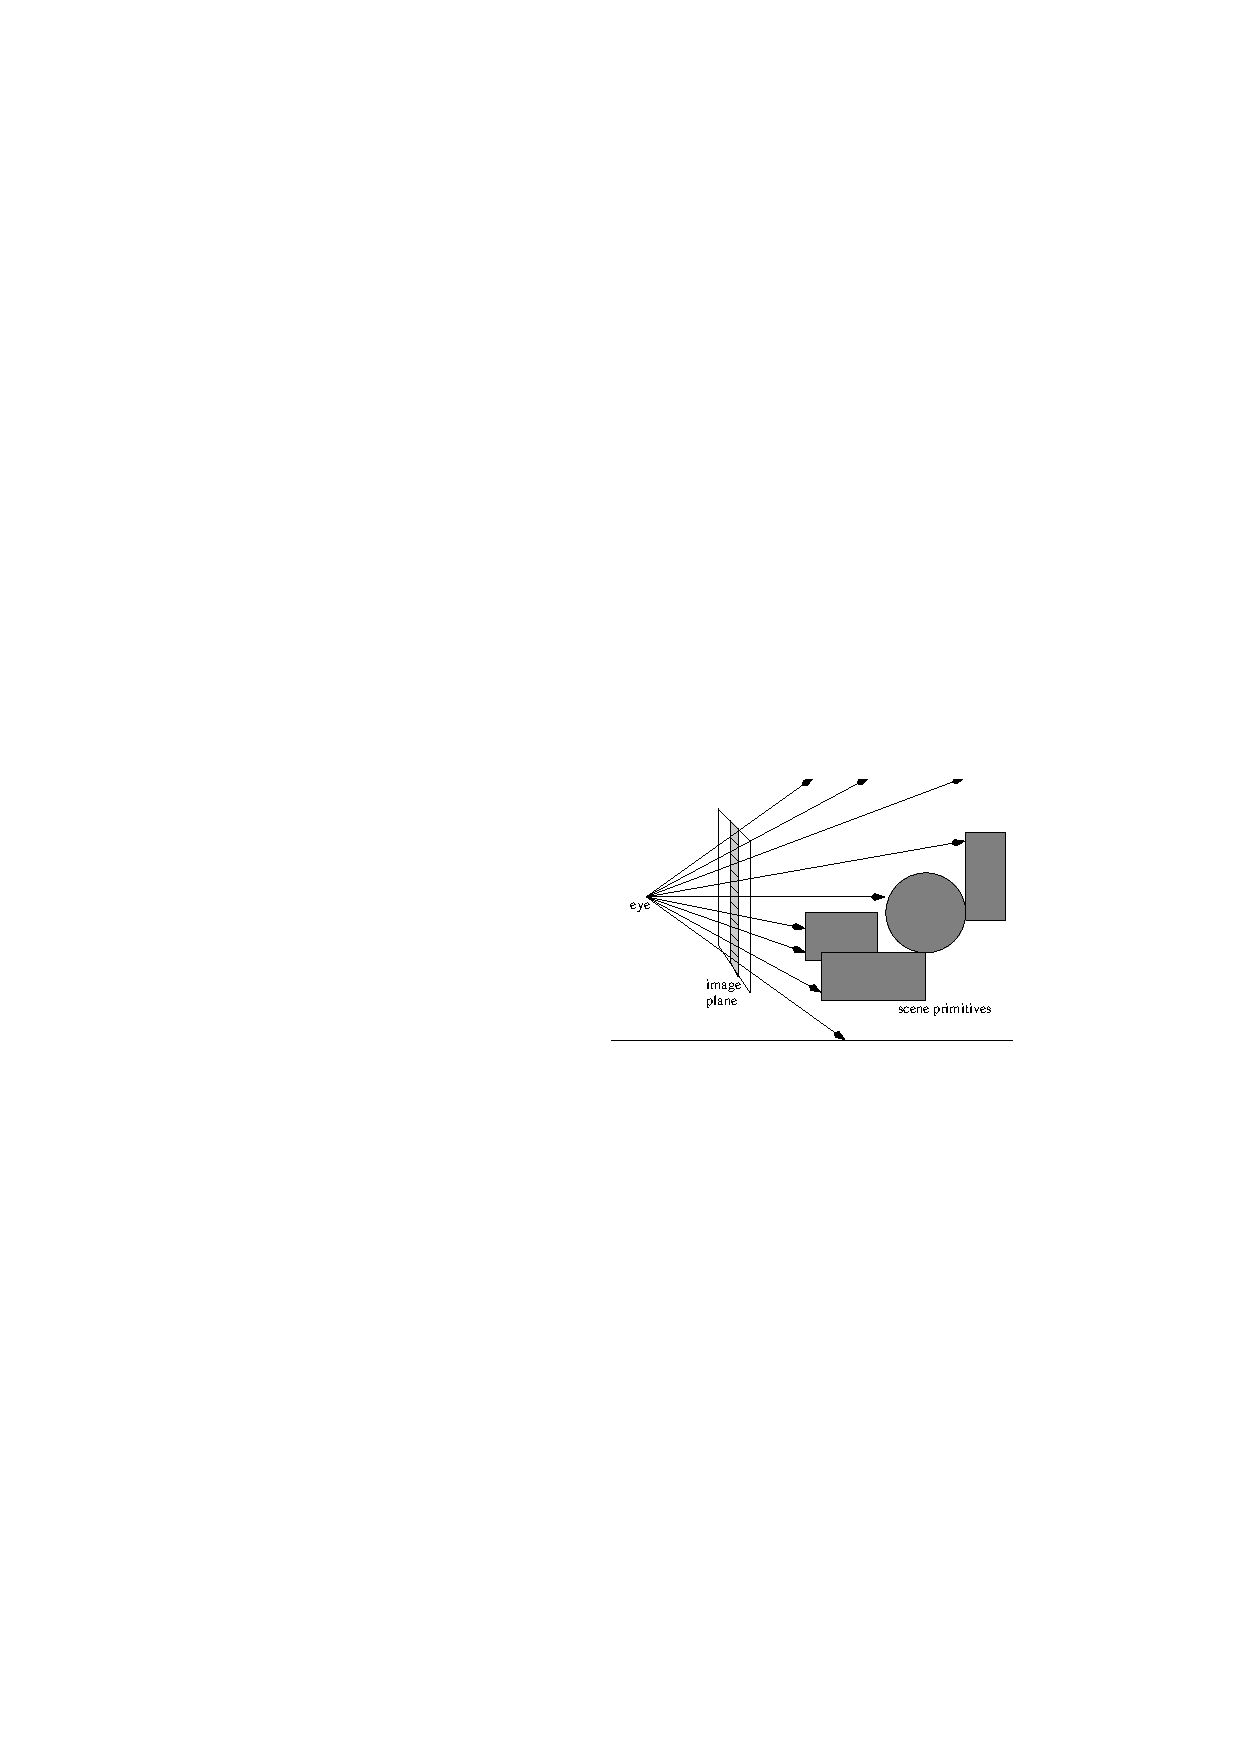
\includegraphics[width=0.45\linewidth]{figRayCastB.pdf}}}
			\renewcommand{\thefigure}{\thechapter.\arabic{figure}}
			\caption[Ray Casting]{\emph{The principle of ray casting: In order to compute an image of a scene, ``primary rays'' are shot from the camera, through each pixel of the virtual image plane, and cast into the scene (a). For each such ray, the closest object hit by this ray is determined by intersecting the ray with the geometric primitives that make up the scene (b).}} 
			\label{fig:ray_casting}	%% label for entire figure
		\end{figure}

	\item[Light and Visibility] \hfill \\

		In order to correctly support shadows, light sources only contribute to the incident illumination if the hit point is not occluded from the position of the respective light source, which is checked by tracing a shadow ray towards the direction of the light source.
		Additional to direct illumination from light sources, illumination from arbitrary other directions (e.g. from the reflection and refraction directions for specular effects) can be considered by casting a secondary ray into the respective direction and recursively evaluating the light being transported along this rays. This recursive evaluation then proceeds in exactly the same way as for the primary ray. Of course, these secondary rays can in turn trigger another recursion level of new rays, etc.


	\item[Ray-Surface Interaction] \hfill \\
		The appearance of a surface is determined by the how the surface interact with the light. The properties of the surface are typically abstracted as the \textit{material} which is actually a parameterized descriptions of the appearance at each point on the surface. These properties are modelled mathematically by the \textit{Bidirectional Reflectance Distribution Function} (BRDF). This function takes the incoming light direction, the outgoing light direction and the point hit by the light as the inputs, returns the amount of energy reflected by the surface at that point. 

	\item[Recursive Ray Tracing] \hfill \\
		The rays shot from the camera (termed as ''primary rays'') can be reflected about the surface normal at the intersection point and transmitted when intersect the transparent object, spawning secondary rays that ray-tracer need to recursively call the ray-tracing routine to trace, the contribution of the secondary rays will be added to the primary rays. 

		\begin{figure}[htp] 
			\centering 
			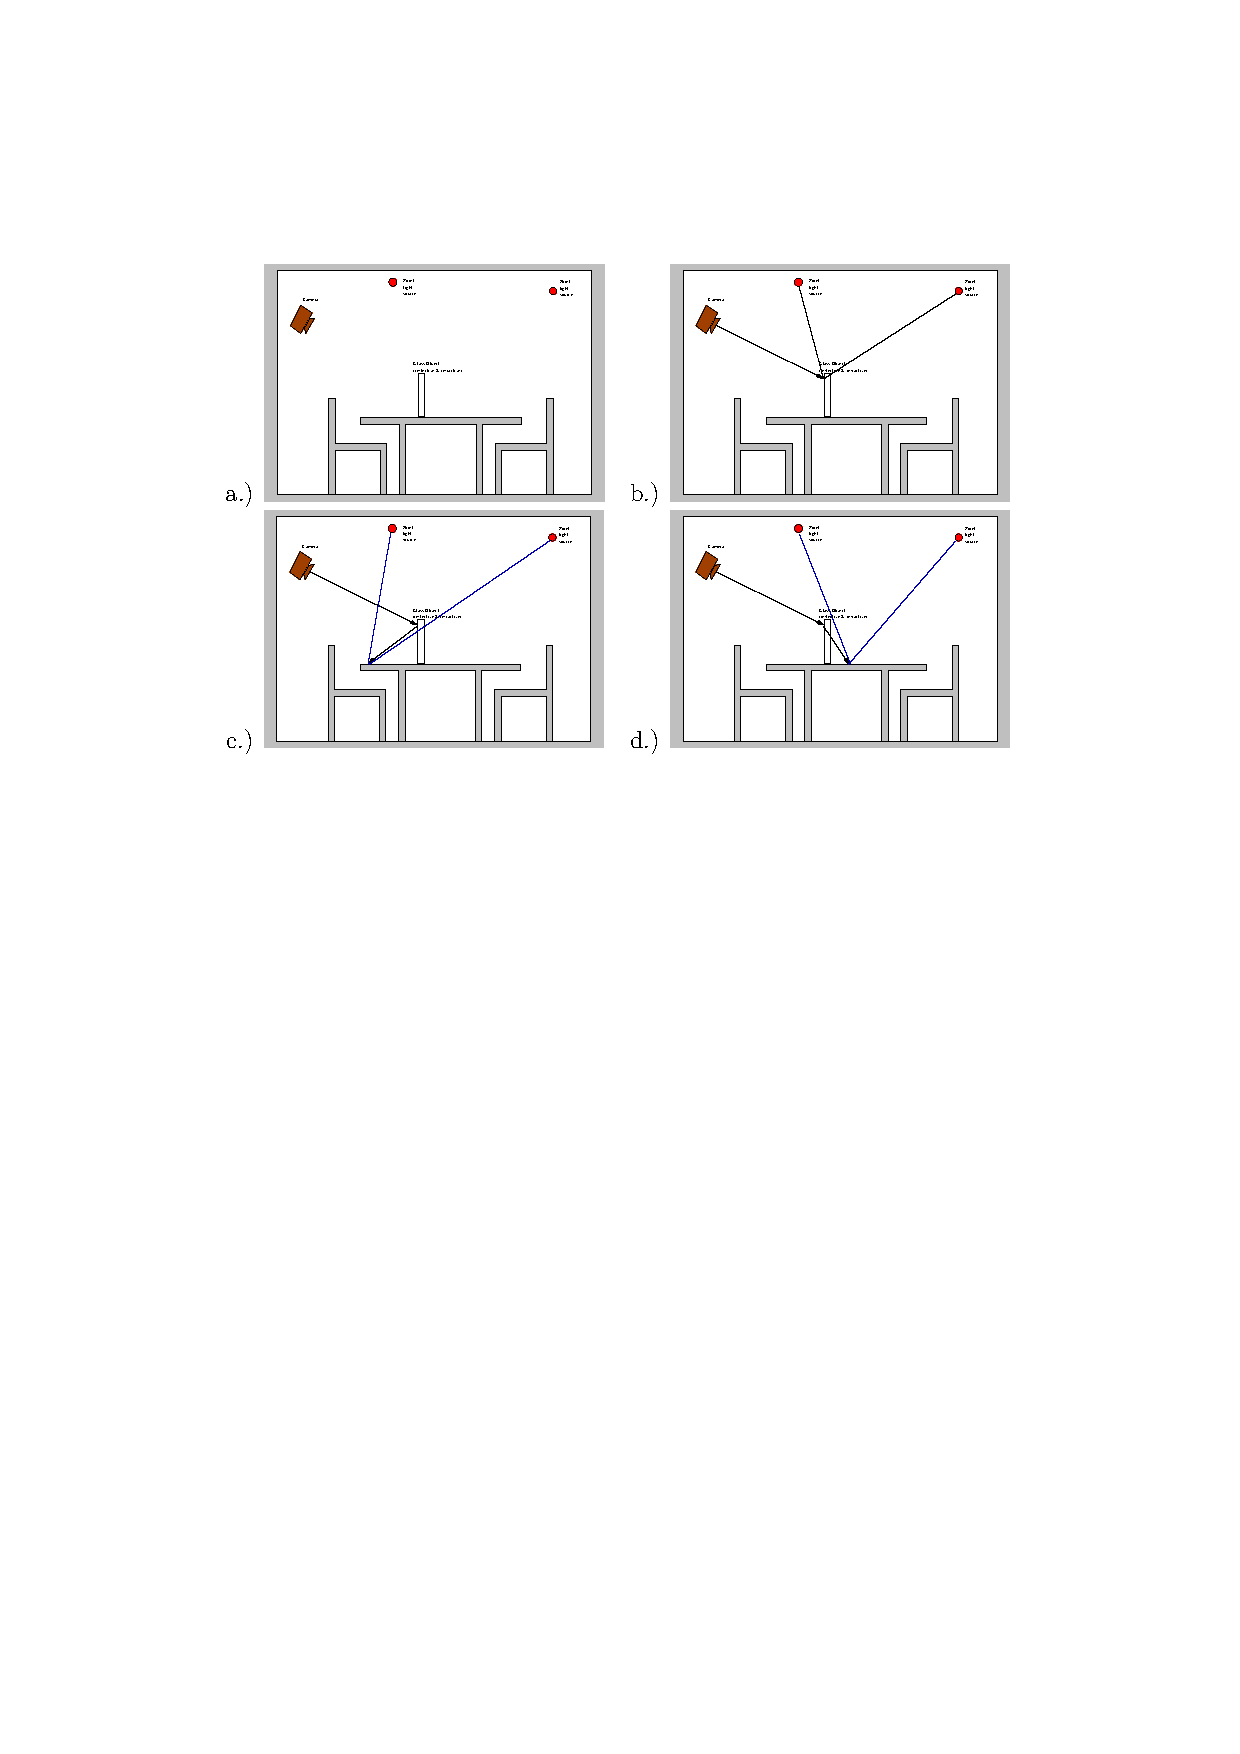
\includegraphics[scale=0.9]{figRayTracingRoom.pdf} 
			\renewcommand{\thefigure}{\thechapter.\arabic{figure}}
			\caption[Recursive Ray Tracing]{}
			\label{fig:ray_tracing_room} 
		\end{figure}

\end{description} 

\newpage

\section{Acceleration Structures}
The ray shooting algorithm which only uses a list of of all objects in the scene is also called a naive ray-shooting algorithm. It is a linear search process that tests the ray with all the objects and choose the one with the closest intersection found, if such an object exists. Thus the time complexity is \( O(n) \). As the scene complexity grows, the application using naive RSA runs unacceptably slowly. The straightforward approach to accelerate ray shooting algorithm is to reduce the number of unnecessary ray-primitive intersection tests. Thus we introduce the concept of acceleration structure.

The AS essentially is a kind of data structure which stores the spatial relationships of the geometric objects in the scene, thus it is also called \emph{spatial data structure}. The idea behind it is similar to accelerating other type of searching problem, if we can establish a kind of index structure which offers the relationship between the elements before performing query, lots of unnecessary tests can be skipped and the performance can be boosted. Over the last 20 years, many different kind of acceleration structures have been developed, however in principle these techniques mainly differ in whether they hierarchically organize the scene primitives (as done by Bounding Volume Hierarchy), or whether they subdivide the space into a set of non-overlapped voxels (as done by kd-trees or grids).  

Generally speaking, acceleration structures can be classified into two types by the approaches they adopt: spatial subdivision and object subdivision. Spatial subdivision approach subdivides the space into regions, hierarchically organizes the geometric objects which fall in the same spatial region into an object called \emph{cell}, and maintains the spatial relationships between the cells. When the ray shooting algorithm is performing, we test the ray against the cells instead of actual geometric objects, if the intersection is found, we go deep in this cell for further test, otherwise this cell will be skipped cause there is no chance that the ray can hit the any geometric objects in this cell, a significant number of intersection tests will be reduced. The most widely-used spatial subdivision structures are uniform grid and kd-tree. 

Object subdivision approach, on the other hand, logically breaks the object in the scene down into a set of objects groups, similar with building a scene graph. For example, a desk can be broke down into four legs and a surface, this forms a hierarchy structure to represent a desk object. If a ray does not hit the desk's bounding volume, there is no chance that the ray hits any parts of the desk and they will be culled, otherwise the ray will be recursively tested against each part of desk. The most widely-used structure of this approach is bounding volume hierarchy (BVH).

% Grid 
\subsection{Grid}

% What is Grid

% Grid Construction

% Grid Traversal

%Bounding Volume Hierarchy
\subsection{Bounding Volume Hierarchy}

% What is BVH 
Bounding volume hierarchy (BVH) are an acceleration structure based on primitive subdivision. The primitives are partitioned into a hierarchy of non-overlapped sets. In the hierarchy, the leaf node keeps the bounding volume of the attached primitive as the nodes' bounding volume, it also stores the actual primitive reference, while the interior node stores the bounding volume of its children node. When a ray is traversed through the tree, any time it misses a node's bounding volume, the entire sub-tree rooted by that node will be skipped. There are two important properties of BVH structure, one is that each primitive referenced by the hierarchy only once,  thus it will not be tested against the ray multiple times; the other one is that the memory consumption to represent the BVH is bounded. Figure ~\ref{fig:BVH} shows a simple scene and its corresponding BVH tree.

\begin{figure}[htp] 
	\fbox{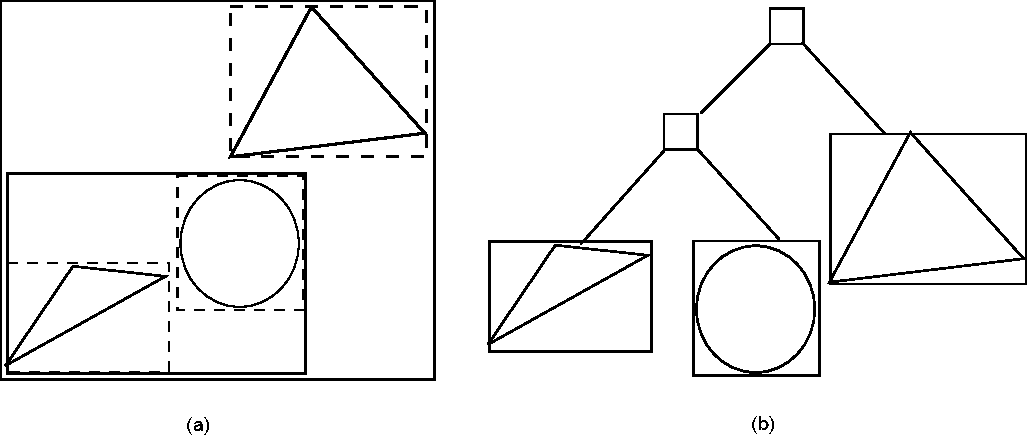
\includegraphics[scale=0.8]{figBVH.pdf}} 
	\renewcommand{\thefigure}{\thechapter.\arabic{figure}}
	\caption{Bounding Volume Hierarchy for a Scene}{(a) A simple scene containing several objects. The bounding boxes of the primitives are shown by dashed lines. The smaller triangle and the sphere are grouped together with a bounding box before being bounded by the bounding box that is corresponding the entire scene (both shown in solid box). (b) The corresponding bounding volume hierarchy, the root node stores the bounding box of the entire scene, it has two children node here, one is a leaf node with the bigger triangle attached, the other one is an interior node that encompasses the sphere and smaller triangle as leaf nodes. }
	\label{fig:BVH} 
\end{figure}

% BVH Construction 
\subsubsection{BVH Construction}
\label{subsubsec:bvh_construction}

Several stages are needed in the BVH construction process. 

\SetAlFnt{\small}
%\IncMargin{1em}
\begin{algorithm} 
	\SetKwInOut{Input}{input} \SetKwInOut{Output}{output}
	\Input{The collection of the primitives in the scene}
	\Output{The root node of BVH tree} 

	\Begin{
	\textit{Initialize the array for primitives}
	\textit{Recursively build BVH tree}
	\textit{Map the BVH tree to a compact linear representation}
	}
	\caption{Build BVH from primitives}
	\label{algo:BVH_construction} 

\end{algorithm}

Firstly, we and store centroid of the bounding box, the complete bounding box and the reference to the primitive for each primitive into an array as a working buffer.

Next, a partition procedure will be performed to split the primitive into two subsets and recursively build the BVH for the subsets. This produces a binary tree where each interior node holds the pointer to  its children nodes and each leaf node holds the references to one or a list of primitives. The partition step can be more complex, given \(n\) primitives, there are \( 2^n - 2 \) possible partitions, while many of them may lead to suboptimal BVH. Generally we choose the partition plane along a coordination axis, meaning that there are about \( 6n \) candidate partitions ( \( 2n \) partitions for each axis ). We use one axis of the three to place the partition. In practice, the axis with the greatest variation of bounding box centroid for the current set of primitives is a good choice. When choosing the position to place the partition plane, a general goal is to select a partition that doesn't have too much overlap of the bounding boxes of the two resulting primitive sets, this is based on the fact that overlapping of two primitive sets will cause the traversal of both children subtrees requiring more computation clipping collection of primitives. 

There are several schemes to choose where to place the partition: a simple method is to partition at the midpoint of the primitives' centroids along the splitting axis. However, this method may result a substantial overlap of two primitive subsets with certain distribution of primitives. Another straightforward but more adaptive partition scheme is to partition the primitives into two subsets with equal number of primitives. These two primitive partitioning approaches above can work well for some distributions of primitives, but they often choose the partitions leading to more nodes of the tree being traversed by the ray and hence unnecessarily ray-primitive intersection computations at rendering time. A more widely-used scheme used by best current algorithms for building acceleration structures are based on the ``surface area heuristic''  (SAH) model which provides a well-grounded cost model used to determine which of a number of partitions of primitives leading a better BVH for ray-primitive intersection tests. The SAH model will be discussed in depth in the chapter. As the partition has been fixed, we generate two interior nodes and classify the geometries into them by testing the primitives against the bounding volume the generated nodes.

Instead of only store the root node of the tree and visiting the nodes by manipulating the pointers, it is an important optimization to store the BVH tree into a compact linear array in depth-first array. This representation makes the BVH traversal more cache-friendly thus improves the overall performance. In the memory, the first child of each interior node is right next to the interior node, for the second child node, the offset to it is stored explicitly in the data structure of BVH tree node. See Figure ~\ref{fig:bvh_linear_layout} for an illustration of the topology of BVH tree nodes and its representation in memory.   

\begin{figure}[htp] 
	\centering 
	\fbox{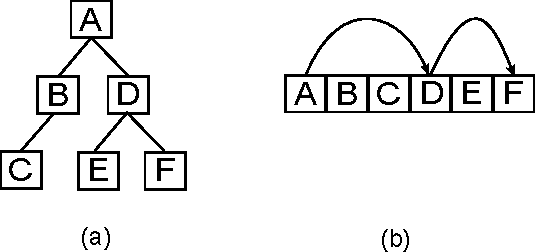
\includegraphics[scale=0.8]{figBVHLinearLayout.pdf}}
	\renewcommand{\thefigure}{\thechapter.\arabic{figure}}
	\caption[Linear Layout of a BVH in memory]{(a) The topology of the nodes in BVH tree. (b) The memory layout of the nodes of the BVH tree. The nodes are stored in depth-first order.}
	\label{fig:bvh_linear_layout}
\end{figure}

% BVH Traversal
\subsubsection{BVH Traversal}
\label{subsubsec:bvh_traversal}
The traversal of BVH is a simple process, the ray is tested against the bounding volume of the node in the tree from the root node which represents the entire scene down to the leaf nodes.  If an intersection occurs (including the case that the ray starts inside of the node), for an interior node, a down traversal is performed to visit the children nodes and save the far node onto a stack, for a leaf node, each primitive will be tested against the ray. If there is no intersection, no further test will be be performed in the current sub-tree and the next node to be visited is retrieved from the stack (or finish the traversal if the stack is empty). The intersection test between the ray and bounding volume is fast, take bounding box for example, ray-box is fast ray-slab test \cite{kk1986}. 

\SetAlFnt{\small}
%\IncMargin{1em}
\begin{algorithm} 
	\SetKwData{RootNode}{root} \SetKwData{Node}{node} \SetKwData{Stack}{stack}
	\SetKwData{NodeIndex}{nodeIndex} 
	\Begin{
		\tcp{Initialise the stack, push the root node} 
		push $root$ onto $stack$  
		\While{true} {
			\tcp{Retrieve the top node of the stack}	
			$node \longleftarrow stack[nodeIndex]$ \\	
			\If{the ray intersects the bounding box of the current node} {
				\If{$node$ is leaf node} { 
					\textit{Intersect ray with primitives in leaf node} 	
				}
				\Else{
					\textit{Put far BVH node on $stack$, advance to near node}
				}
			}
			\Else{
				\If{$stack$ is empty} {break}
				\textit{Advance $nodeIndex$}
			}
		}
	}
	\caption{BVH Traversal}
	\label{algo:bvh_traversal} 
\end{algorithm}


% KD-Tree
\subsection{KD-Tree}
Before introducing kd-tree, a short introduction to \textit{Binary Space Partitioning} (BSP) tree has to be made. A BSP tree is a data structure developed in the purpose of solving the hidden surface removal problems in computer graphics. The binary space partitioning is a process of adaptively and recursively subdivide the voxel of the scene into irregular sized regions with a chosen split plane until a termination criteria has been satisfied. Different scheme of choosing the split plane leads to two major variants of BSP tree, polygon-aligned form and axis-aligned form. The polygon-aligned form chooses the plane aligning the polygon in the scene as the split plane, while axis-aligned form always chooses the planes perpendicular to a certain coordinate axis. The kd-tree is actually the axis-aligned form of the BSP tree which makes both traversal and construction of the tree more efficient. We will focus on kd-tree here in this thesis.

\begin{figure}[H] 
	\centering
	\fbox{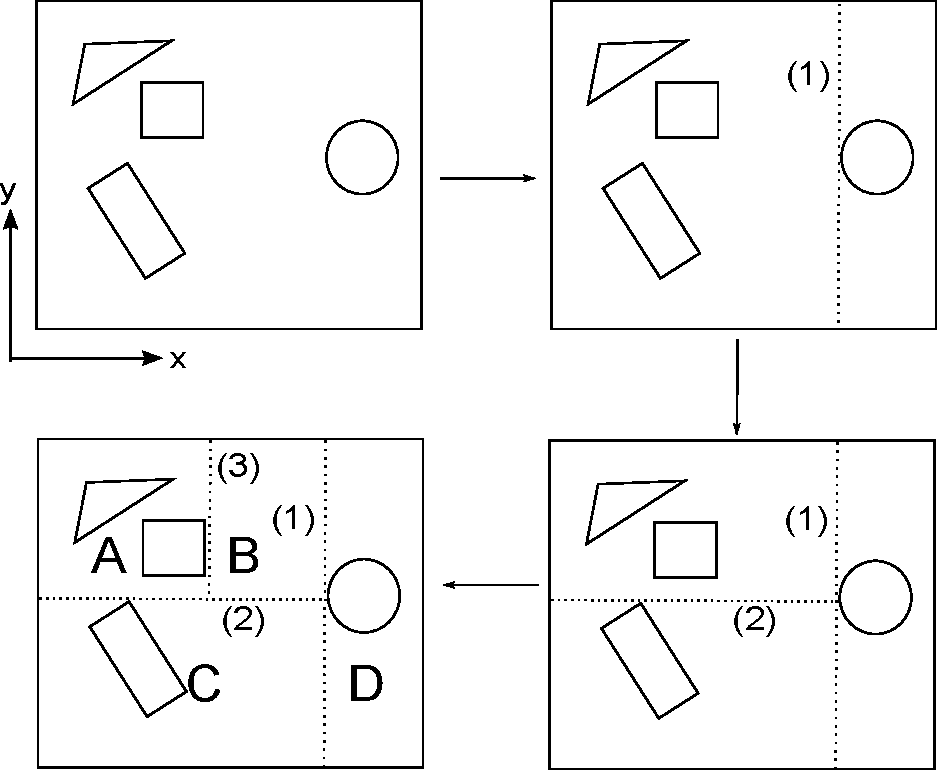
\includegraphics[scale=0.8]{figKDTreeSubdivide.pdf}} 
	\renewcommand{\thefigure}{\thechapter.\arabic{figure}}
	\caption[2D view of the subdivision of a scene]{The top view of a scene which is recursively subdivided by the split planes (shown in dashed lines and labeled by numbers) into several small regions (labeled by the letters).}
	\label{fig:kd-tree_subdivide} 
\end{figure}

Figure ~\ref{fig:kd-tree_subdivide} provides an overview of how the scene is recursively subdivided along one of the coordinate axes. In the figure, a scene is recursively subdivided by 3 split planes. Initially, the entire scene as the root node of the tree, the first split is along the \(x\) axis and it subdivides the scene into two regions. Then the left region is refined a few more times with the number 2 splitting plane. In the subdivision process, some criteria such as which axis is used to place the splitting planes,  at which position along the axis the plane is placed and at what point subdivision terminates can all substantially affect the performance of the kd-tree in practice.  

%then termination test is performed to see if the partitioning should be stopped, in this case we continue subdivision, thus the newly generated voxels left and right become the children of the root node. Next step we split the left node into two voxels and assume the termination criteria has been satisfied, the subdividing should be stopped here, thus the new child nodes becomes the leaf node of the kd-tree, as labeled by ``A'' and ``E''. Any Internal node has the references to its child nodes and the leaf nodes will contain a list of primitives which fall in the spatial region covered by the leaf node. The primitive which straddles a split plane will belong to all the nodes it intersects with.

\begin{figure}[H]
	\centering
	\fbox{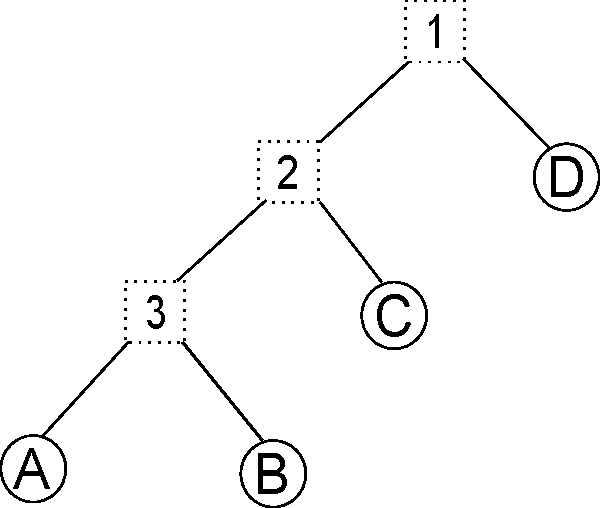
\includegraphics{figKDTreeSubdivideTree.pdf}} 
	\renewcommand{\thefigure}{\thechapter.\arabic{figure}}
	\caption[KD-Tree representation of a simple scene]{The kd-tree built from the scene in Figure \ref{fig:kd-tree_subdivide}}
	\label{fig:kd-tree_subdivide_tree} 
\end{figure}

% Why kd-tree
%KD-Trees are useful data structure for the searching problems which RSA requires, nearest neighbor search (NNS). Because it essentially sorts the primitives into two sets, the one in front of the split plane and those behind, relative to the origin of a given ray, we can determine the which set of primitives is nearer to the origin, and which is further. To find the closest primitive hit by the ray, we simply perform a down-traversal in a front-to-back order on the kd-tree built from the scene, when the leaf node is reached, a linear search will be required to find the primitive with the minimum distance to the origin of the ray. Furthermore, since the split planes are orthogonal to the coordinate axis, the intersection test between the ray and splitting plane has been greatly simplified. 

% KD-Tree Representation
\subsubsection{KD-Tree Data Representation}
As a special case of binary tree, the node of kd-tree has the similar representation. Each interior node has to contain the following three data fields: 
\begin{itemize}\itemsep1pt
	\item{Split axis: which axis is used to to place the splitting plane for this node}
	\item{Split position: the position of the splitting plane along the splitting axis}
	\item{Reference to children nodes: information associates to the children of this nodes}
\end{itemize}
While each leaf nodes only contains the reference to the collection of primitives attached to it. Both leaf nodes and interior nodes share a common data filed which is a flag indicating the this node is a leaf or interior. 

In practice all these data fields can be put in a compact data structure which consume 8 bytes (assuming the system uses 4-byte floating point values and pointers) regardless if the node is an interior or a leaf node using the \textbf{union} in C/C++ programming language. They share the same memory location using one bit of data to indicate it is leaf node or interior and the node-specific data is encoded into a 4-byte unsigned integer value. For interior node, 

\begin{lstlisting}[caption=Data layout of kd-tree node, label=lst:kd-tree_node]
	struct KDTreeLeaf{
		unsigned int flag; 
		// bits 0..30  	: offset bits
		// bit 31(sign) : flag whether node is a leaf  
	}
	struct KDTreeInterior{
		float split; 
		unsigned int flag; 
		// bits 0..1 	: splitting dimension
		// bits 2..30 	: offset bits
		// bit 31(sign) : flag whether node is a leaf
	}
	union KDTreeNode{ 		
		struct KDTreeLeaf;
		struct KDTreeInterior; 
	}
\end{lstlisting}

% kd-tree construction
\subsubsection{KD-Tree Construction}
\label{subsubsec:kd-tree_construction}
A kd-tree construction essentially is a process of recursively subdivide the current spatial region into two subregions with a certain axis-aligned split plane that is selected using a particular strategy. The construction process starts with the extend of the entire scene. Initially, the root node is leaf node, and all newly generated nodes are also leaf nodes, when a node is split by split plane, it will become an interior node, and the objects associated with it will be sorted to into its two new descendants. 

The recursion will be terminated when a certain termination criteria is reached. Commonly we use the maximum depth of the recursion or a pre-defined threshold of the number of the primitives attached to a leaf node as the termination criteria. In practice, the value \(8 + 1.3\log(N)\) is found a reasonable maximum depth of the tree for a variety of scenes \cite{ph2004}.The construction of kd-tree is described in pseudo-code in Algorithm \ref{algo:kd-tree_construction}.


% Begin the algorithm: kd-tree construction
\SetAlFnt{\small}
\begin{algorithm}[H]

	\SetKwData{triangleList}{\(T\)}
	\SetKwData{triangleListLeft}{\(T_{L}\)}	
	\SetKwData{triangleListRight}{\(T_{R}\)}

	\SetKwData{voxel}{\(V\)}
	\SetKwData{voxelLeft}{\(V_{L}\)}
	\SetKwData{voxelRight}{\(V_{R}\)}
	\SetKwData{currentNode}{\(node\)}
	\SetKwData{currentBox}{\(box\)} 
	\SetKwData{splitPlane}{\(p\)}

	\SetKwFunction{CalcBounds}{\ProcNameSty{CalcBounds}}
	\SetKwFunction{FindSplitPlane}{\ProcNameSty{FindSplitPlane}}
	\SetKwFunction{ClassifyTriangles}{\ProcNameSty{ClassifyTriangles}}
	\SetKwFunction{SAHCost}{\ProcNameSty{SAHCost}}
	\SetKwFunction{KDTreeBuildRec}{\ProcNameSty{KDTreeBuildRec}}
	\SetKwFunction{BuildRec}{\ProcNameSty{BuildRec}}
	\SetKwFunction{Terminate}{\ProcNameSty{Terminate}}
	\SetKwFunction{CreateLeafNode}{\ProcNameSty{CreateLeafNode}}
	\SetKwFunction{CreateNode}{\ProcNameSty{CreateNode}}
	
	\myfunc \BuildRec{\triangleList, \voxel} \newline 
	\Begin {
		\If {\Terminate{\triangleList, \voxel}}	{
			\Return \CreateLeafNode{\triangleList}\; 
		}
		
		\splitPlane = \FindSplitPlane{\triangleList, \voxel}\;
		(\voxelLeft, \voxelRight) = Split \voxel with \splitPlane\;
		(\triangleListLeft, \triangleListRight) = \ClassifyTriangles{\triangleList, \voxelLeft, \voxelRight, \splitPlane}\;
		
		\Return \CreateNode{\splitPlane, \BuildRec{\triangleListLeft, \voxelLeft}, \BuildRec{\triangleListRight, \voxelRight}}\;
	}

	\myalgblankline
	
	\myfunc \KDTreeBuildRec{\triangleList} \newline
	\Begin {
		\voxel = \CalcBounds{\triangleList}\;
		\Return \BuildRec{\triangleList, \voxel}\;
	}

	\caption{Recursive KD-tree construction}
	\label{algo:kd-tree_construction}
\end{algorithm}


As shown in the above algorithm, in each partition of the current node, a split plane has to be selected, this is done by the function \emph{FindSplitPlane}. For a kd-tree, a split plane can be positioned arbitrarily, as long as they are perpendicular to one of the \( {x, y, z} \) axis. However, different strategy of choosing the split plane may lead to a considerable performance gap up to a factor of two of more when traversing the built kd-tree \cite{havran200}. More detail will be discussed in chapter 3. 

\subsubsection{KD-Tree Traversal}
\label{subsubsec:kd-tree_traversal}
%kd-tree traversal
% 1. Motivation
% 2. Describe with figures
% 3. Pseudocode 

Given a ray \(R\) and a kd-tree, the kd-tree traversal is a procedure that identify the sequence of the kd-tree leaves intersected by the ray. There are several types of traversal algorithms developed, such as sequential, recursive and those with neighbor-links. Due to the simplicity, here we only describe the recursive traversal algorithm. The traversal is in a top-down fashion, starting from the root node, recursively descends the branches of the kd-tree along the ray path. Before going into any details of the ray traversal algorithm, a few terminologies have to be introduced, For each interior node the ray visits, the mutual position of the origin of a ray and the axis-aligned box \( AB(s) \) of this node has to be considered. The first configuration is when the origin of a ray is located outside, also known as ``the ray with external origin'', and the other one is when the origin of the ray is inside the \( AB(s) \), we call it ``the ray with internal origin''. When a bounding box is intersected by a ray \( R \), there are two important points along the ray path which can be expressed by two signed distance. The point where \( R \) enters the bounding box is called \emph{entry point}, corresponding to the \emph{entry signed distance}. The point where R leaves the bounding box is called \emph{exit point}, corresponding to the \emph{exit signed distance}. 

When the ray enters a kd-tree node (one traversal step), the intersection between the ray and the bounding box associating to the current node creates a parameter interval \( t_{near}, t_{far} \) which are the signed distance of the entry and exit point. Intersecting the ray with bounds of the entire scene (the tree's root node) gives the initial \( t_{near}, t_{far} \), then the parameter interval is updated incrementally during the traversal. If the ray misses the overall bounding box ( \( t_{near} > t_{far} \) ), then the traversal can exit immediately. 

If the current node is a leaf node, each primitive attached is tested against the ray and update a parameter \( t_{closest} \) to find the closest intersection point. 

If the current node is an interior node, it has to determine which of the two children the ray enters first. We calculate the parametric distance \(d\) to the splitting plane of the node in the same manner as was done in computing the intersection of a ray and axis-aligned plane for the ray-bounding box test, \( d = (t_{split} - r_{origin}[dim]) / r_{dir}[dim] \), and then compare \(d\) to the current ray segment \( t_{near}, t_{far} \). If the ray segment lies completely on one side of the splitting plane ( \( d >= t_{far}\ or\ d <= t_{near}\) ), the subtree on the other side can be skipped immediately and the traversal will continue to proceed to the corresponding child voxel. Figure \ref{fig:kd-tree_traversal_one_child} shows some configurations of this case. 

\begin{figure}[hpt]
	\centering
	\fbox{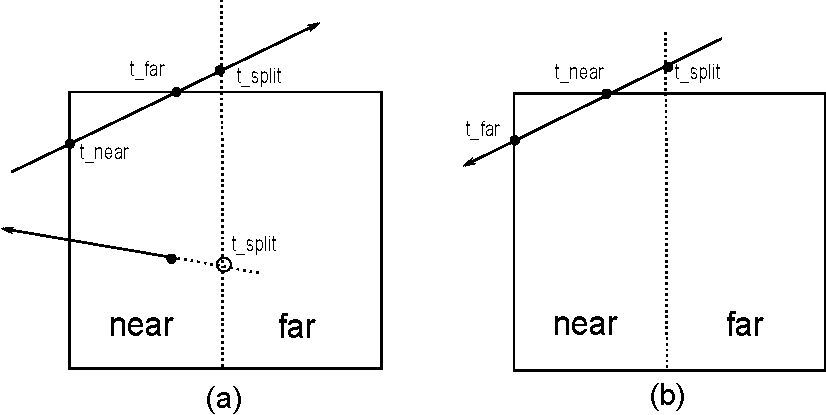
\includegraphics{figKDTreeTraversalOneChild.pdf}}
	\renewcommand{\thefigure}{\thechapter.\arabic{figure}}
	\caption[KD-tree traversal proceed only one child node] {Two cases where the traversal will only proceed one child node. }
	\label{fig:kd-tree_traversal_one_child}	%% label for entire figure
\end{figure}
 
If none of the children nodes can be culled, the position of the ray's origin with respect to the splitting plane is enough to determine which of the child node is closer in turn should be visited first, figure \ref{fig:kd-tree_traversal_children} illustrate this case.  

\begin{figure}[H]
	\centering
	\fbox{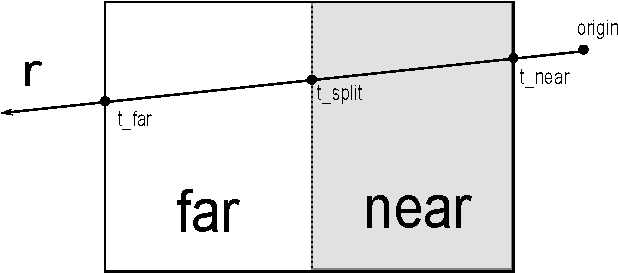
\includegraphics{figKDTreeTraversalChildren.pdf}}
	\renewcommand{\thefigure}{\thechapter.\arabic{figure}}
	\caption[KD-tree traversal proceed both children nodes] {The children nodes are labeled as ``near'' and ``far'' by checking \( t_{split} - r_{origin}[dim] \). If it is positive, the ray enters the left node first; otherwise the right node is the ``near'' node.  The parameter interval for traversal the ``near'' and ``far'' node are \( t_{near}, t_{split} \), \( t_{split}, t_{far} \) repectfully. }
	\label{fig:kd-tree_traversal_children}	%% label for entire figure
\end{figure}

Figure \ref{fig:kd-tree_traversal} shows the basic process of ray traversal through the tree. 
\begin{figure}[hpt]
	\centering
	\fbox{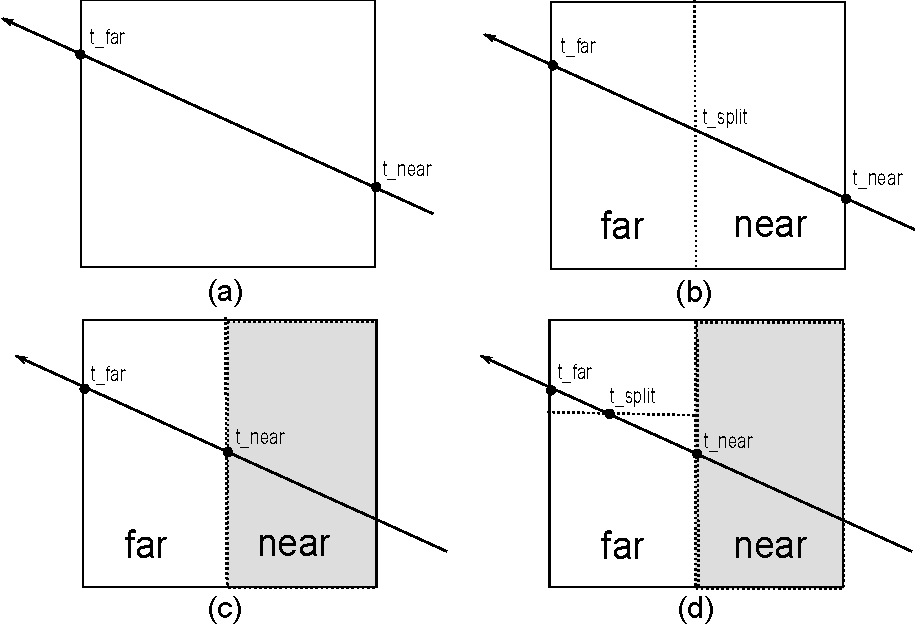
\includegraphics[width=\linewidth]{figKDTreeTraversal.pdf}}
	\renewcommand{\thefigure}{\thechapter.\arabic{figure}}
	\caption[Traversal of Ray Through the KD-Tree.]{(a) The ray intersects against the bounding box of the kd-tree. The two intersection points can be simply represented by a parametric range \([t_{near}, t_{far}]\). (b) Assume this node is an interior node, it is necessary to consider the two children nodes. The node that the ray enters first is labeled as ``near'', corresponding the range \([t_{near}, t{split}]\). If the near node is leaf node which contains geometric primitives, ray-primitives intersection tests will be performed; otherwise, its children nodes will be processed. (c) If no intersection found in the near node, then the far node (on the left) is processed. (d) The traversal process will continue in a depth-first, front-to-back order, until the closest intersection is found or the ray exits the tree.	
	} % end of caption
	\label{fig:kd-tree_traversal}	%% label for entire figure
\end{figure}

% The algorithm 
\SetAlFnt{\small}
\begin{algorithm}[H]
	% Variables 
	\SetKwData{ray}{\(r\)}
	\SetKwData{rayOrigin}{\(r.origin\)}
	\SetKwData{rayOriginDim}{\(r.origin[node.dim]\)}
	\SetKwData{rayDirection}{\(r.dir\)}
	\SetKwData{rayDirectionDim}{\(r.dir[node.dim]\)}
	\SetKwData{tNear}{\(t_{near}\)}
	\SetKwData{tFar}{\(t_{far}\)}
	\SetKwData{tClosest}{\(t_{closest}\)}
	\SetKwData{tHit}{\(t_{hit}\)}
	\SetKwData{D}{\(d\)}	

	\SetKwData{rootNode}{\(rootNode\)}
	\SetKwData{node}{\(node\)}
	\SetKwData{nodeSplit}{\(node.split\)}
	
	% Functions
	\SetKwFunction{KDTreeTraversalRecFunc}{\ProcNameSty{KDTreeTraversalRec}}
	\SetKwFunction{TraversalRecFunc}{\ProcNameSty{TraversalRec}}
	\SetKwFunction{RayBoxIntersectionFunc}{\ProcNameSty{RayBoxIntersection}}
	\SetKwFunction{RetrieveFarNodeFunc}{\ProcNameSty{RetrieveFarNode}}
	\SetKwFunction{RetrieveNearNodeFunc}{\ProcNameSty{RetrieveNearNode}}
	
	\myfunc \KDTreeTraversalRecFunc{\ray, \rootNode} \newline
	\Begin{
		{\tNear, \tFar} $\leftarrow$ \RayBoxIntersectionFunc{\ray, \rootNode}\;
		\If {\tNear > \tFar} {
			\tcp{The ray misses the bounding box}
			\Return\; 
		}
		
		\TraversalRecFunc{\rootNode, \tNear, \tFar}\; 
	}
	
	\BlankLine \BlankLine 

	\myfunc \TraversalRecFunc{\node, \tNear, \tFar} \newline
	\Begin{
		Initiailise \tClosest to the maximum distance\; 
		\If { \node is leaf node} { 
			Intersect all the primitives in the node against the ray\; 
			\Return \tClosest\;
		}
		\D $\leftarrow$ (\nodeSplit - \rayOriginDim) / \rayDirectionDim \;
		\If {\D <= \tNear} {
			\tcp{Cull the ``near'' node}
			\Return \TraversalRecFunc{ \RetrieveFarNodeFunc{\node}, \tNear, \tFar}\; 
		}
		\ElseIf {\d >= \tFar} {
			\tcp{Cull the ``far node}
			\Return \TraversalRecFunc{ \RetrieveNearNodeFunc{\node}, \tNear, \tFar}\;
		}
		\Else {
			\tcp{Need to proceed both children nodes}
			\tHit $\leftarrow$ \TraversalRecFunc{\RetrieveNearNodeFunc{\node}, \tNear, \D}\;
			\If {\tHit <= \D} {
				\Return \tHit\; 
			}
			\Return \TraversalRecFunc{\RetrieveFarNodeFunc{\node}, \D, \tFar}\;
		}
	}
	\caption{Recursive KD-Tree Traversal}
	\label{algo:kdtree_traversal_rec}
\end{algorithm}






%-------------------------

%-------------------------
% Chapter 3: Ray-Tracing with KD-Tree

\chapter{Efficient KD-Tree For Ray-Tracing}
\setcounter{figure}{1}      % reset the figure counter
\label{ch:effiecient_kd-tree}

\section{KD-Tree Construction Algorithm} 
The general kd-tree construction algorithm has been presented in the previous text, in this section, more advanced techniques adopted on the construction of kd-tree will be discussed in depth.

\subsection{Surface Area Heuristic}

In the algorithm \ref{algo:kd-tree_construction}, a recursive construction of kd-tree in top-down fashion has been presented, essentially all kd-tree construction algorithm follow the same scheme. The key operation in the construction of kd-tree is to effectively picking a split plane in every subdivision. There are several best known methods for positioning the splitting plane in the kd-tree:

\begin{comment} 
\begin{figure}[htp] 
    \centering 
    \fbox{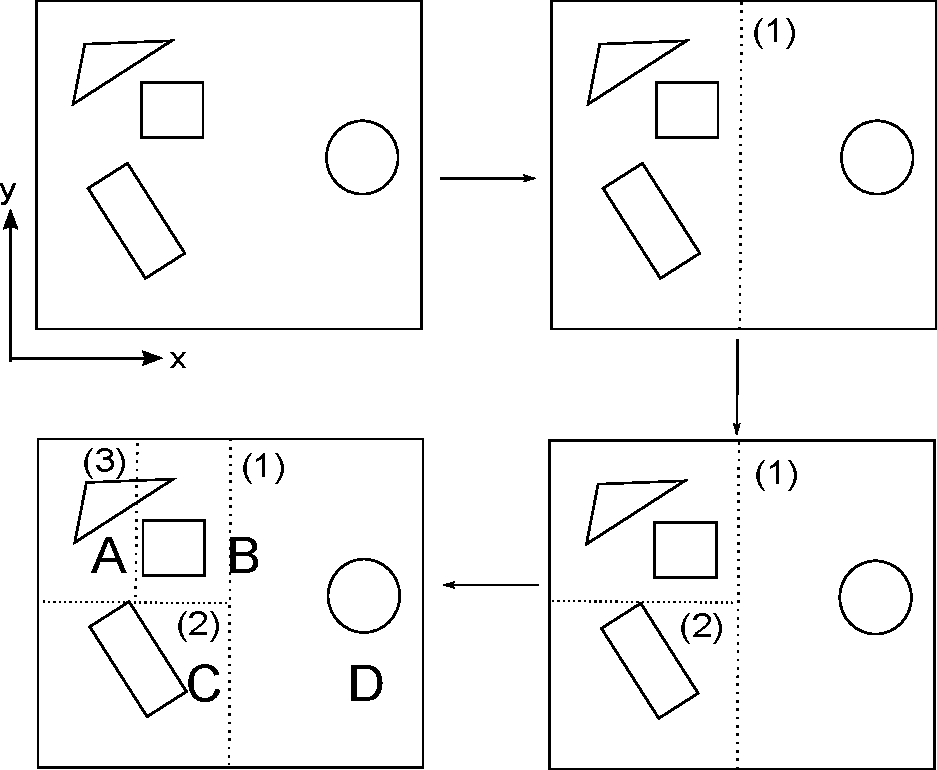
\includegraphics[width=\linewidth]{figKDTreeSubdivideSpatialMid.pdf}} 
    \renewcommand{\thefigure}{\thechapter.\arabic{figure}}
    \caption[The scene with the spatial median subdivision]{\emph{ The scene with the spatial median subdivision}}
    \label{fig:kd-tree_subdivide_spatial_mid}
\end{figure}
\end{comment}

% what is SAH
In \cite{havran2000}, Vlastimil Havran introduced ``surface area heuristic'' (SAH), which provides a well-grounded cost model that estimates the average cost of traversing an arbitrary ray through the kd-tree. The estimated cost is used to determine which split plane among a number of split candidates should be chosen in order to lead to a more efficient acceleration structure for ray-primitives testing. Most of the best current acceleration structures' building algorithms are based on SAH cost model. 

The SAH cost model provides an estimation of the computational expense of performing ray intersection tests, including the time spent traversing nodes of the tree and the time spent on ray-primitive intersection test for a subdivision of primitives. The goal for the kd-tree construction algorithm to follow is to minimize the total cost, particularly for a greedy algorithm like algorithm \ref{algo:kd-tree_construction}, the goal is to minimize the cost for each subdivision step.

For each subdivision step, we have to decide whether to make the current region a leaf node with all of the overlapping primitives attached or refine the region to create two subregions. In the first case, any ray that passes through this region will be tested against all of the primitives leading to a cost of 
	$\displaystyle\sum\limits_{i=1}^N C_{isect}(i)$

Where N is the number of primitives and \(C_{isect}(i)\) is the cost of computing the intersection between the ray and the \(i\)th primitive. 

For the other case which is to split the region, the cost can be modeled with the following equation:

\begin{equation} 
	\label{eq:CostOneStep}
	C(A, B) = C_{trav} + p_{A} \cdot \sum\limits_{i=1}^{N_{A}} C_{isect}(a_{i}) + p_{B} \cdot \sum\limits_{i=1}^{N_{B}} C_{isect}(b_{i})
\end{equation}

Where the \(C_{trav}\) is the cost of traversing the interior node, \(p_{A}\) and \(p_{B}\) are the probabilities of the ray passing through each of the child nodes. \(a_{i}\) and \(b_{i}\) are the primitives attached on the two children nodes, and \(N_{A}\) and \(N_{B}\) are the number of the primitives overlapping with of the subregions respectively. 

The probabilities \(p_{A}\) and \(p_{B}\) can be computed using the ideas from geometric probability. A convex volume A contained in another convex volume B, the conditional probability that a random ray passing through B will also pass through A is the ratio of their surface areas, \(s_{a}\) and \(s_{b}\): 
\begin{equation} 
	p(A|B) = \frac{s_{A}}{s_{B}} 
\end{equation}

\subsection{KD-Tree Construction With SAH} 
As described in the chapter \ref{ch:background}, the kd-tree is built with a recursive top-down algorithm. At each step, we have an axis-aligned region of space and a set of primitives that overlap the region. Either the region is split into two subregions and turned into an interior node, or a leaf node is created with the overlapping primitives, terminating the recursion.  
% why is the SAH-based kd-tree beneficial for the ray-tracing
The strategy of choosing the split plane in the kd-tree construction process may have considerable impact on the performance of ray-tracer. An \mynaive approach is to place the split plane at the middle of region along certain axis splitting each node in half at each level and generating a balanced binary tree. Similar to the binary search tree, this approach is beneficial when the goal is to quickly figure out in which leaf node a certain point locates. However, in addition to quickly query the geometric primitive hit by the ray, the goal of kd-tree traversal is to find the closest intersection point. With the strategy of picking the spatial middle point as the split plane, it is likely to create the leaf nodes which contain lots of geometr as the distribution of geometry is not taken into account. The disadvantage of this approach is that whenever a ray traverses through a leaf node, it has to test for intersection with all of the primitives even there is no chance they could intersect. To minimize the redundant intersection tests, the distribution of geometry has to be somehow encoded into the kd-tree built from a certain scene to provide heuristic information for the ray tracer in kd-tree traversal stage. It is optimal to maximize the space of the leaf node which contains little geometry and minimize the space that contains more geometry. Figure \ref{fig:kd-tree_subdivide_spatial_mid_vs_sah} shows the different effect when traversing the tree built by two different approaches. 

\begin{figure}[htp] 
    \centering 
    \fbox{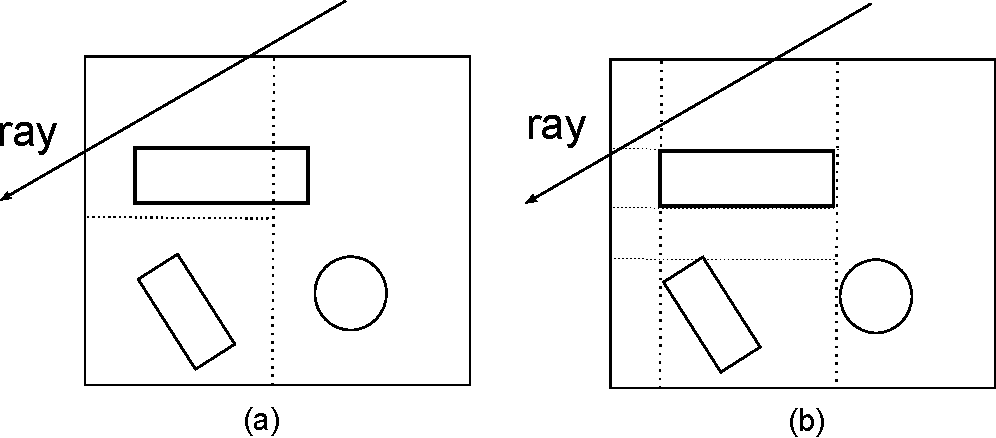
\includegraphics[scale=0.8]{figKDTreeSubdivideSpatialMidVsSAH.pdf}} 
    \renewcommand{\thefigure}{\thechapter.\arabic{figure}}
    \caption[Spatial median split and SAH-based split]{(a) The scene is subdivided using the spatial middle point and the created leaf nodes will cause redundant intersection tests. (b) The scene is subdivided based on the SAH cost model resulting a higher quality kd-tree. When a ray traverse through the kd-tree, it can quickly skip those leaf nodes without performing intersection tests since the empty region is isolated from the region that contains more geometry.}
    \label{fig:kd-tree_subdivide_spatial_mid_vs_sah}
\end{figure}

% SAH-based kd-tree construction 
With the definition of the SAH cost model, we can easily adopt the SAH in the kd-tree construction algorithm. As shown in the algorithm \ref{algo:kd-tree_construction_sah}. 

The termination criteria of the SAH-based algorithm is more stable when to stop subdivisions. As the cost of a leaf node can be modeled as \(C_{leaf} = K_{isect}\lvert T \rvert\), the subdivision will be terminated when the further split of this leaf node has higher cost than not splitting at all. 

The ``FindSplitPlaneSAH'' function takes the list of triangles \(T\), the voxel that to be split \(V\) and an axis \(k\) as the input parameters, outputs the split with the minimum cost. However, this process is not trivial compares to the spatial median splitting which only costs \mycomplexityconst. To calculate the cost for each split candidates, we have to determine the number of primitives of both left and right child \(N_{L}\) and \(N_{R}\). This can be done by classifying the triangle list which cost \mycomplexityn. Therefore the overall complexity for finding the optimal split algorithm is \mycomplexitysqrtn. 


\SetAlFnt{\small}
\begin{algorithm}[H]
	\SetKwData{true}{\(true\)}
	\SetKwData{false}{\(false\)}

	\SetKwData{tri}{\(t\)}
	\SetKwData{triangleList}{\(T\)}
	\SetKwData{triangleListLeft}{\(T_{L}\)}	
	\SetKwData{triangleListRight}{\(T_{R}\)}
	\SetKwData{triangleListLeftNum}{\(\lvert\)\triangleListLeft\(\rvert\)}
	\SetKwData{triangleListRightNum}{\(\lvert\)\triangleListRight\(\rvert\)}

	\SetKwData{voxel}{\(V\)}
	\SetKwData{voxelLeft}{\(V_{L}\)}
	\SetKwData{voxelRight}{\(V_{R}\)}
	\SetKwData{currentNode}{\(node\)}
	\SetKwData{currentBox}{\(box\)} 
	
	\SetKwData{splitPlane}{\(p\)}
	\SetKwData{splitPlaneBest}{\(p_{best}\)}
	\SetKwData{splitPlaneCan}{ \{ \(p_0, p_1, \dots\) \} }
	\SetKwData{splitPlaneList}{\(P\)}
	
	\SetKwData{axis}{\(k\)}
	
	\SetKwData{cost}{\(C\)}
	\SetKwData{costMin}{\(C_{min}\)}

	\SetKwFunction{CalcBounds}{\ProcNameSty{CalcBounds}}
	\SetKwFunction{CalcBoundEdge}{\ProcNameSty{CalcBoundEdge}}
	\SetKwFunction{FindSplitPlaneSAH}{\ProcNameSty{FindSplitPlaneSAH}}
	\SetKwFunction{CalcSplitCandidates}{\ProcNameSty{CalcSplitCandidates}}
	\SetKwFunction{ClassifyTriangles}{\ProcNameSty{ClassifyTriangles}}
	\SetKwFunction{SAHCost}{\ProcNameSty{SAHCost}}
	\SetKwFunction{Terminate}{\ProcNameSty{Terminate}}
	
	\myfunc \ClassifyTriangles{\triangleList, \voxelLeft, \voxelRight, \splitPlane} \Return (\triangleListLeft, \triangleListRight) \newline 
	\Begin {
		\triangleListLeft = \triangleListRight = \(\phi\)\;		
		\ForAll {\tri \(\in\) \triangleList} {
			\If {\tri overlaps with \voxelLeft} {append \tri to \triangleListLeft\;}
			\If {\tri overlaps with \voxelRight} {append \tri to \triangleListRight\;}
		}
	}
	
	\myalgblankline
	
	\myfunc \FindSplitPlaneSAH{\triangleList, \voxel, \axis} \Return \splitPlaneBest \newline
	\Begin {
		\ForAll{\tri \(\in\) \triangleList} {
			\splitPlane = \CalcBoundEdge{\CalcBounds{\tri}, \axis}\;
			Append \splitPlane to split plane list \splitPlaneList\; 
		}
		\ForAll{\splitPlane \(\in\) \splitPlaneList} {
			(\voxelLeft, \voxelRight) = split \voxel with \splitPlane\; 
			(\triangleListLeft, \triangleListRight) = \ClassifyTriangles{\triangleList, \voxelLeft, \voxelRight, \splitPlane}\;
			\cost = \SAHCost{V, \splitPlane, \triangleListLeftNum, \triangleListRightNum}\;
			\If {\cost < \costMin} {
				(\costMin, \splitPlaneBest) = (\cost, \splitPlane)\;
			}
		}
	}
	\caption{Find the optimal split plane based on SAH}
	\label{algo:kd-tree_construction_sah}
\end{algorithm}

\subsubsection{Fast KD-tree Construction in \mycomplexitynlogn} 
It is easy to observe that the algorithm \ref{algo:kd-tree_construction_sah} is inefficient mainly due to the computation of the SAH cost for each split candidate requires the \(N_{L}\) and \(N_{R}\) which again triggers an iteration over the triangle list. In \cite{wh2006}, Wald and Havran introduced a fast SAH-based kd-tree construction algorithm whose time complexity is \mycomplexitynlogn. The improved algorithm takes the advantage of the increment of the split plane position, as the split plane ``sweeping'' over the split candidates,  the \mynumtrileft and \mynumtriright can be updated using a incremental scheme. Consider a split plane \mysplitplane in an axis \mydimension and its position is denoted as \mysplitplanepos, there is a certain number of triangles lying on the left, right side of it, which is also can be called as the number of end, starting planes respectively. Let us denote the number of starting triangles for the split plane \mysplitplane as \mynumtristartp, the number of end triangles \mynumtriendp.   

Let us consider \(n\) split planes candidates \{ \mysplitplanen{0} \}, along one fixed axis \mydimension, and assume that all the planes are sorted in ascending order. For the first split plane candidate \mysplitplanen{0} which has the minimum coordinates value, there will be no triangle on the left, all the triangles are lying on the right side of it. 

\begin{displaymath} 
    N_{L}^{(0)} = 0 \qquad N_{R}{(0)} = N
\end{displaymath} 

As the split plane ``sweeping'' from split plane \mysplitplanen{i-1} to \mysplitplanen{i}, the \mynumtrileft and \mynumtriright will change as follows: 
\begin{enumerate} 
    \item The triangles started at \mysplitplanen{i-1} will intersect with left voxel \myleftchildbox. 
    \item The triangles ended at \mysplitplanen{i} will no long intersect with right voxel \myrightchildbox 
\end{enumerate}

Therefore the \mynumtrileft and \mynumtriright can be updated incrementally using the following equations: 
\begin{equation}
	N_{L}^{i} = N_{L}^{i-1} + p^{+}
	N_{R}^{i} = N_{R}^{i-1} - p^{-}
    \label{eq:SweepUpdate}
\end{equation}

Follow this updating rule, all the \mynumtrileft and \mynumtriright of all the split planes candidates can be computed incrementally by iterating over the all the possible split position \mysplitplanen{i}. Firstly, we need to fix a dimension \mydimension, for this \mydimension, we go through all the triangles \mytriangle and generate the split candidates associated with \mytriangle, for each candidate, an ``event'' will be generated and stored. The ``event'', \myevent = (\myeventt, \myeventp, \myeventk, \myeventtype), is actually defined as a data structure which contains four data fields: a reference to the triangle whose bounding box's face defines the split candidate, the coordinate value of split position and the event type. The reference to \mytriangle can be simply an index of it, denoted as \myeventt, the plane position is a float-point value, denoted as \myeventp, the dimension \mydimension, and event type, \myeventtype, is an enumeration of several flags to indicate the relation between the triangle referenced in this event and the split plane this event corresponds to, start event and end event. According to the definition, a start event always corresponds to a split position at minimum face of the triangle's bounding box, while end event will be generated by a split plane at the position of the maximum face. Three lists of events against all axises will be generated by iterating over all the triangles, and will be eventually merged into one list \myeventlist\ in an interleaved fashion respect to the dimension, this obviously requires the event structure to have an tag to indicate which axis the event corresponds to. Secondly, each of the list of consecutive events for the same axis needs to be sorted, and the comparison of two events \(e_{a}\) and \(e_{b}\) is shown as equation \ref{eq:EventCompare}. For those events with different positions, they will be sorted by ascending the coordinate values, for those events with same positions, they will be sorted by comparing the event type, that is, the end event will precede the start event. Suppose there are two adjacent triangles which share one vertex, only one split plane candidate will be generated at the vertex, while there will be two events to be stored, one end event references the triangle that is ``before'' the plane, and one start event references the triangle that is ``beyond'' the plane. So by counting the start and end events, the \mynumtrileft and \mynumtriright can be easily determined regarding a certain plane.

% Event Comparison
\begin{equation} 
    e_{a} < e_{b} = \left\{ 
        \begin{array}{ll}
            true & (a_{p,k} < b_{p,k}) \vee ( (a_{p,k} = b_{p,k}) \wedge (a_{type} < b_{type}) ) \\
            false & otherwise
        \end{array} \right.
        \label{eq:EventCompare}   
\end{equation} 

To compute the \mynumtrileft and \mynumtriright for each split plane candidates \mysplitplanen{i} using the sorted event list to find the best one, we consider all dimensions in one loop, for each dimension, a separate \mynumtrileftk{k}, \mynumtrirightk{k}\ needs to be stored. For each dimension, we perform the ``sweeping'' using the above incremental updating scheme. We firstly consider the sequence of the \mysplitplanen{i}-related events, count the end and start events to determine the number of start and end triangles \mynumtristartip{i} and \mynumtriendip{i}. Then the \mynumtrileft and \mynumtriright for the split planes can be maintained and updated by applying the update equations. Once the \mynumtrileft, \mynumtriright are determined, the SAH cost is readily to compute and we can find the best split plane by choosing the one with minimum cost. The algorithm is shown as follows: 

\SetAlFnt{\small}
\begin{algorithm}[H]
    
    \SetKwData{vari}{i}
    \SetKwFunction{FindBestPlane}               {FindBestPlane}
    \SetKwFunction{SplitCandidates}             {SplitCandidates}
    \SetKwFunction{SAHCost}                     {SAHCost}
    \SetKwFunction{SAH}                         {SAH}
    \SetKwFunction{SplitBox}                    {SplitBox}
    
    \textbf{pre:} E has been sorted.   
    \myfunc \FindBestPlane{\myeventlistk{x,y,z}, \myvoxel, \mynumtri} \Return \mybestsplitplane\\
    \Begin {
        (\mycostmin,\mysplitplane) = (\myinfty,\myemptyset)\; 
        \ForAll {\mydimension\ in \{x, y, z\}} {
            \{start: all triangles are right side only for each k\}\\ 
            \mynumtrileftk{k} = 0, \mynumtrirightk{k} = \mynumtri\;  
            \For {$i \leftarrow 0$ \KwTo \mynumeventlist} {
                % get the plane in current k
                \mysplitplane = (\myeventlistpi{$i$}, \myeventlistki{$i$})\;
                \mynumtristartp = \mynumtriendp = 0\;
                \{iterate over all plane candidates.\}\\
                \While{$i$ \(<\) \mynumeventlist\ \(\wedge\) \mysplitplanek = \myeventlistki{$i$} \(\wedge\) \mysplitplanep = \myeventlistppi{$i$} \(\wedge\) \myeventlistti{$i$} = \myeventtypeend} { 
                    inc \mynumtriendp\;
                    inc $i$;
                }
                
                \While{$i$ \(<\) \mynumeventlist\ \(\wedge\) \mysplitplanek = \myeventlistki{$i$} \(\wedge\) \mysplitplanep = \myeventlistppi{$i$} \(\wedge\) \myeventlistti{$i$} = \myeventtypestart} {
                    inc \mynumtristartp\;
                    inc $i$\;
                }
                \mynumtrirightk{k} -= \mynumtriendp\; 
                \mycostp = \SAH{\mysplitplane,\myvoxel,\mynumtrileftk{k},\mynumtrirightk{k}}\;
                \If {\mycostp\ \(<\) \mycostmin} {
                    (\mycostmin,\mysplitplane) = (\mycostp,\mysplitplane)\;
                } 
                \mynumtrileftk{k} += \mynumtristartp\;     
            }
        }  
        \Return \mycostmin\; 
    } 
    \caption{The \mycomplexityn\ algorithm of finding the best SAH split plane}
    \label{algo:FindBestPlaneON} 
\end{algorithm}

After finding the best split plane \mybestsplitplane, classifying the triangle list into two sub-lists is another important step in one recursion step. Since the best split in current recursion is found using a sorted events list, we have to find a way to compute two sub-lists of events \myeventlistleft and \myeventlistright, and more importantly, to maintain the ascending order of them so that they can become inputs for the following recursion step without performing any sorting. As the input event list \myeventlist is sorted, and the best split plane \mybestsplitplane\ has been found, if an event is of end type and its position is less than the \mybestsplitplane, the triangle this event references must be in the left sub-list of triangle \mylefttrilist, symmetrically, the triangle referenced in a start event with a greater position than the \mybestsplitplane must belongs to the \myrighttrilist. The remaining triangles should be counted in both \mylefttrilist and \myrighttrilist. The triangle classification algorithm is shown as following: 

\SetAlFnt{\small}
\begin{algorithm}[H]
    \SetKwFunction{ClassifyTriangles}           {ClassifyTriangles}
    \myfunc \ClassifyTriangles{\mytrilist,\myeventlist,\mybestsplitplane} 
        \Return \mylefttrilist,\myrighttrilist,\myeventlistleft,\myeventlistright\\ 
    \Begin {
        \ForAll{\myevent\ \myopin\ \myeventlist} {
            \If {\myeventtype=\myeventtypestart\  
                    \myopand\ \myeventk=\mybestsplitplanek\  
                    \myopand\ \myeventp\myopless\mybestsplitplanep} {
                 
                    set \mytriflagsarray{\myeventt}.\mytriflagleft\;
                  
                } 
           \If {\myeventtype=\myeventtypeend\ 
                    \myopand\ \myeventk=\mybestsplitplanek\ 
                    \myopand\ \myeventp\myopgreater\mybestsplitplanep} {
                    
                     set \mytriflagsarray{\myeventt}.\mytriflagright\;
                 }
        } % End of ForAll event
        \ForAll {\mytriangle\ \myopin\ \mytrilist} {
            \If {\mytriflagsarray{\mytriangle}.\mytriflagleft is set} {
                \mylefttrilist\ appends \mytriangle\; 
            }
            \If {\mytriflagsarray{\mytriangle}.\mytriflagright is set} {
                \myrighttrilist\ appends \mytriangle\; 
            }
        } % End of \ForAll triangles
        
        \ForAll {\mydimension\ \myopin\ \{x, y, z\}} {
            \ForAll {\myevent\ \myopin\ \myeventlistk{\mydimension}} {
                \If {\mytriflagsarray{\myeventt}.\mytriflagleft} {
                    \myeventlistleftk{\mydimension} appends \myevent\;
                } 
                \If {\mytriflagsarray{\myeventt}.\mytriflagright} {
                    \myeventlistrightk{\mydimension} appends \myevent\;
                } 
            }
        } % End of \ForAll k
    } % End of Begin
    
    \caption{The triangle classification algorithm in \mycomplexityn.}
    \label{algo:ClassifyTriangles} 
\end{algorithm}

\subsection{Optimizations of KD-tree Construction on CPU}

% Multi-core CPU parallel

\subsubsection{Parallelization}
\label{subsubsec:parallelization}


There have been many attempts to parallelize the SAH-based KD-tree construction on CPU. Many approaches follow the same parallel pattern \cite{msk2007}, \cite{p2006}. As the builder often starts with a large amount of geometry, the initial phase of the algorithm is a breadth-first top-down hierarchy construction process to organize all the geometry primitives into a few nodes at the top of their hierarchies using a single thread. In this phase the spatial median \cite{zhou2008} or geometry count median \cite{msk2007} partitioning strategy are preferred over expensive full SAH cost computation in many known approaches. When the number of nodes at a level meets or exceeds the number of cores, the algorithm switches to depth-first node-parallel construction. Each subtree is assigned to a separate thread and perform the SAH partition independently. 

A ``nested'' parallel algorithm was introduced in \cite{c2010} providing a pattern utilizing both node-level and geometry-level parallelism. At the top levels of the tree, the major functions in the sequential algorithm have been parallelized, these functions include \textbf{FindBestPlane}, \textbf{ClassifyTriangles} and \textbf{FilterGeometry}. 

\paragraph{FindBestPlane} 
The parallelized version of \textbf{FindBestPlane} is a process with 3-passes which are \textbf{PreScan}, \textbf{Push}, \textbf{SAHScan}. Given the array of generated events, we first decompose the event list into \(n\) contiguous chunks, the memory for each chunk is allocated in each thread. In the \textbf{PreScan} phase, each of the \(n - 1\) thread counts the number of start and end events in its corresponding chunk as there is no need to scan the last chunk, yielding \(N_{L}\) and \(N_{R}\) specifically for the chunk. The \textbf{Push} is a prefix sum process that sums up the total \(N_{L}\) and \(N_{R}\) of previous chunk to the total of the current chunk, yielding correct \(N_{L}\) and \(N_{R}\) at the beginning of each chunk. This \textbf{Push} phase can be implemented with both sequential and parallel algorithm, however, it is not very beneficial to parallelize it using a multi-core CPU that is only with a few cores. For the \textbf{SAHScan} phase, each thread performs an iteration over its corresponding chunk of events, calculating the \(N_{L}\) and \(N_{R}\) and finding the minimum SAH cost within the current chunk. A final sequential reduction is required to get the minimum SAH across all of the \(n\) chunks. 

\paragraph{ClassifyTriangles}

\paragraph{FilterGeometry}


% Each processor core can independently The parallelism pattern can be illustrated by the figure \ref{fig:kd-tree_constrcution_parallel_pattern}

\begin{comment}
\begin{figure}[htp] 
    \centering
    \fbox{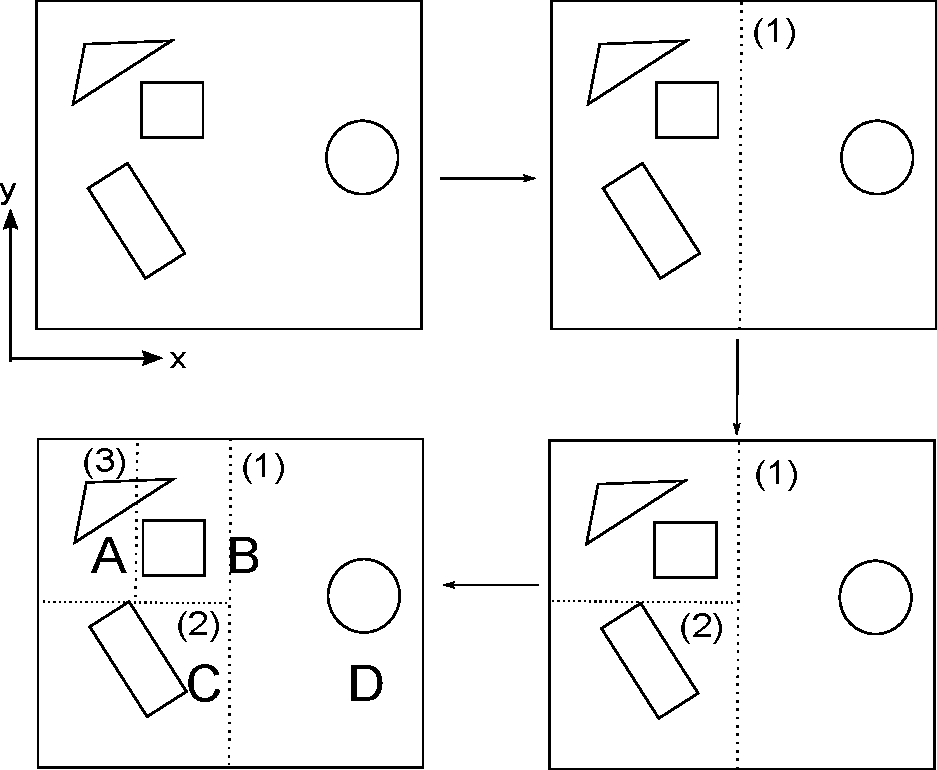
\includegraphics{figKDTreeSubdivideSpatialMid.pdf}} 
    \renewcommand{\thefigure}{\thechapter.\arabic{figure}}
    \caption[The scene with the spatial median subdivision]{\emph{ The scene with the spatial median subdivision}}
    \label{fig:kd-tree_construction_parallel_pattern}
\end{figure}
\end{comment}

\subsubsection{Memory Management}

% Memory access pattern, sequential vs random

% Locality, random access is not cache friendly

% Conventional kd-tree construction algorithm is slow due to the random ram access pattern




%-------------------------

%-------------------------
% Chapter 4: Ray-Tracing with GPU
%\chapter{Ray Tracing Using Graphics Hardware}
\setcounter{figure}{1}      % reset the figure counter
\label{ch:gpu}

After many years of the CPU being the heart of computer system, recent innovations in processor design led to a new type of high-performance processor being easily accessible. Starting with data-parallel graphics processors, these processors have acquired significantly more bandwidth and raw computational power (especially float-point computation) than the CPUs have. CPUs have long been designed mainly focusing on single thread application, the goal of this design is to finish a single computation as quickly as possible. Even though the multi-core design which provides small number of independent processor on a single chip has emerged since 2005. On the other hand, the architecture design focuses on massive parallel application, the processor may have thousands of threads running concurrently with high aggregate computational throughput. Furthermore, as the design goals differ from the CPUs, there are much less space on the chip for caches, branch prediction hardware and out-of-order execution units, given a fixed amount of chip area, GPU chips are able to provide to many more arithmetic logic units (ALUs) than a CPU. While the processor keeps all the ALUs busy execute the computation efficiently in parallel, it can offer approximately ten times as many peak FLOPS as high-end CPUs. Therefore, GPUs have drawn much interest recently in many processing-intensive applications including ray tracing. 

%------------------------------------------
% 
%------------------------------------------

\section{Grpahics Pipeline and Architecture Overview}
Understanding the architecture of GPUs may help developer illustrate the strengths and weaknesses of these processors with respect to major computational patterns, so that developers become able to optimize their applications in a device-friendly way. A short history of the development of modern GPUs is provided in this section to clarify the rationale behind major architectural design decisions, which are massive multi-threading, relative small cache memories compare to CPUs and bandwidth-centric memory interface design. Insights into the historical development will also likely to provide the context needed to understand the algorithms in the following sections. This section starts with the evolution of the graphics pipeline, then the architecture of the general purpose GPU is going to be introduced. 


\subsection{Graphics Pipeline}
The graphics pipeline is the current state of the art method of rasterization-based rendering supported by commodity graphics hardware, it typically accepts some form of representation of a three-dimensional scene as an input, as the data going through each stage which performs certain tasks, rasterized 2D image will be generated as output. 

\paragraph{Fixed-Function Graphics Pipeline}
From the early 1980s to the late 1990s, the leading performance graphics hardware was fixed-function pipelines, where ``fix'' means the functions in the pipeline were configurable but not programmable. Some major graphics application programming interface (API) have become popular in the same era. An API is a standardized software layer that provides with certain form of programming interface (i.e., a collection of library functions) to programmers to enable them to access software services or hardware features for their applications. Programmer can issue commands to instruct graphics hardware to perform certain task via graphics API, such as specifying the geometry data that will be rendered by the hardware, draw some geometry onto the frame buffer or alter certain render states to achieve some effects. Two major graphics API are currently widely used in the industry, OpenGL and Direct3D.

% Describe the data flow here 
Figure \ref{fig:fixed_function_pipeline} shows an example of fixed-function rendering pipeline. The host is the application that uses the graphics pipeline and resides in the systems memory space, while the graphics pipeline is usually implemented in the hardware driver and it can access the dedicated memory on the graphics card. The communications between the host application and graphics pipeline includes commands issues and data transfer between system memory and graphics hardware memory and they can be done via the host interface. 

% @figure: fixed-function graphics pipeline
\begin{figure}[htp] 
    \centering 
    \fbox{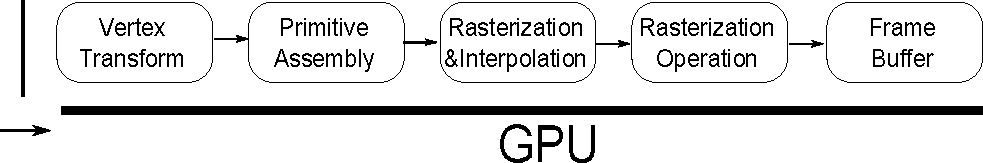
\includegraphics[scale=0.7]{figFixedPipeline.pdf}} 
    \renewcommand{\thefigure}{\thechapter.\arabic{figure}}
    \caption[Fixed-function pipeline]{\emph{Fixed-Function Pipeline}}
    \label{fig:fixed_function_pipeline} 
\end{figure}

% Describe the data type
The modern graphics pipeline is usually designed to take the vertex as the input of data and the vertices are going to be assembled in the pipeline to represent the certain types of geometric primitives (such as triangles) that are going be rendered eventually. The vertices data will be converted into a form that the hardware understands and placed into the vertex cache.  

escribe the major stages in the pipeline
The major stages in the pipeline will be described in the following text. The first important stage in the pipeline is Transform and Lighting (T\&L). This stage takes the attributes of the vertices, such as the positions, normals, colors and texture coordinates) as input, applies the transformations on each vertices and performs the per-vertex shading  according to the light source properties and certain vertex properties. All the output of this stage are per-vertex values.

And the triangle setup stage further creates edge equations that are used to interpolate colors and other per-vertex data across the pixels touched by the triangle in the rendered image. After this stage, it is ready to determine the which pixels are contained in each triangle, this is done by the rasterization stage, at this point, the geometric polygons in the 3D space will be converted to the filled pixels in 2D space, and for each of these pixels, the rasterization process will interpolate per-vertex values neccessary for shading the pixels, including the color, position and texture coordinates that will be shaded (painted) on the pixel.

The next important stage is the shading. As the name implies, the final color of each pixel will be determined in this stage. Many image-based shading techniques and post-processes can be applied here: interpolation of vertex colors, texture mapping, per-pixel lighting calculations and the list goes on and on. 

Following the rasterization stage, the raster operation stage, also known as pixel engines, performs the final raster operation on each pixel. It performs color raster operations that blend the color of overlapping/adjacent objects for transparency and anti-aliasing effects. It also determines the visible objects for a viewpoint and discards the occluded pixels. A pixel becomes occluded when it is blocked by pixels from other objects according to the given new point. 

Finally, the frame buffer interface is responsible for managing the memory reads from and writes to the display frame buffer memory.

For a couple of decades, each generation of hardware and its corresponding generation of API brought incremental improvements to the various stages of the graphics pipeline, however, developers are always asking for more new features than the build-in function can provide. Therefore, an obvious evolution for the graphics pipeline is the programmable graphics pipeline.

\paragraph{Programmable Graphics Pipeline}
Programmable graphics pipeline takes a further step by making certain stages into programmable processors. In graphics pipeline, certain stages do a great deal of floating-point arithmetic on completely independent data, in theses stages certain functions will be applied to each element in a set of data (a stream), such as the transformation on the set of vertices positions and pixels shading calculations on the pixel stream. This data independence is one of the key difference between the design assumption for GPU and CPU, this provides a tremendous opportunity to exploit the data parallelism. 

The specific functions executed in the graphics pipeline may vary with rendering algorithms. Such variation became the motivation to make those pipeline stages programmable. There are two particular stages functions have been turned into programmable processors: the vertex shader and pixel shader. 

The vertex shader programs replace the built-in vertex T\&L stage function in the fix-pipeline and runs once on each vertex of the vertex stream the pipeline receives. Typically they perform the essential transformation of the vertex from 3D world space to 2D projection space and per-vertex shading calculations  according to the properties of vertices and light sources. All the properties of a vertex such as positions, colors and texture coordinates can be manipulated in vertex shader by the customized algorithms.   

The pixel shader program is the alternative to the shader stage in the fixed-function pipeline. The essential task of pixel shader program is to compute the color and other attributes of each pixel in the rendered image, lots of image-based algorithms and techniques are implemented in pixel shader programs to achieve some complex per-pixel effects. 

For all the types of shader programs, the program instances can be running in parallel, since the functions are applied on each independent element in a data stream and independent result is produced. This property has motivated the design of the programmable pipeline stages into massively parallel processors.   

The figure ~\ref{fig:ProgrammablePipeline} shows an example of a programmable pipeline that contains a vertex processor and a pixel processor. It is basically a mix of programmable stages and fix-function stages. Between the programmable stages, there are dozens of fixed-function stages that provides much better performance than the programmable stages and benefits much less from programmability. For example, the rasterization which resides between the vertex shader and pixel shader in the pipeline is a completely hardware-implemented function so that the efficiency can maximized. This design of graphics pipeline offers both extreme performance and flexibility to achieve more sophisticated effects. 

% @figure: programmable graphics pipeline
\begin{figure}[htp] 
    \centering 
    \fbox{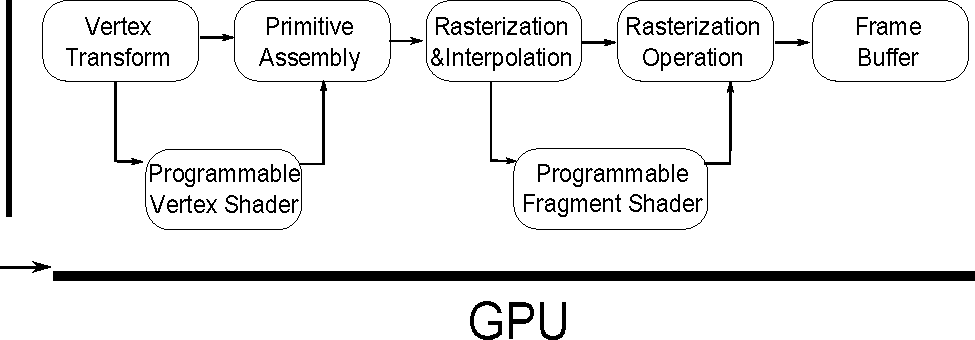
\includegraphics[scale=0.7]{figProgrammablePipeline.pdf}} 
    \renewcommand{\thefigure}{\thechapter.\arabic{figure}}
    \caption[Programmable Graphics Pipeline]{\emph{Programmable Graphics Pipeline}}
    \label{fig:programmable_pipeline} 
\end{figure}

\paragraph{Unified Shaders}
The latest step in the evolution from hardwired pipeline to flexible computational fabric is the introduction of unified shaders, Unified shaders pipeline was first implemented in the ATI Xenos chip for the Xbox 360 gaming console, and the NVIDIA GeoForce 8800 GPU. Instead of separate custom processors of vertex shaders, geometry shaders and pixel shaders, a unified shader architecture provides one large grid of general data-parallel floating-point processors to run all the shader workloads, as illustrated in figure \ref{fig:unified_shaders_pipeline}. This grid of processors can be considered as a pool of unified computational resources, since different applications or even two frames within one application may vary greatly in the demand for various shaders, the array of processors can be allocated dynamically for the demand to achieve a better overall utilization. For example, a video game might begin with a scene with a detail-textured sky without many triangles, this quickly saturates the pixel shaders in a traditional pipeline, while rendering this scene is almost a trivial task. One millisecond later, a scene with highly detailed geometry to draw intricate characters and objects will be rendered, this task will require much more computational power for vertex processing and leave pixel shaders mostly idle. With traditional programmable pipeline, these dramatic changes on in resource demands can vary unpredictably as the players' viewpoint and action change. A unified shader architecture, on the other hand, can allocate a varying percentage of its pool of processor to each shader type. 

% @figure: unified shaders graphics pipeline
\begin{comment}
\begin{figure}[htp]
    \centering 
    \fbox{\includegraphics{.pdf}} 
    \label{fig:unified_shaders_pipeline} 
    \renewcommand{\thefigure}{\thechapter.\arabic{figure}}
    \caption[Unified Shaders Graphics Pipeline]{\emph{Unified Shaders Graphics Pipeline}}
\end{figure}
\end{comment}

\section{General Purpose GPU}
% the motivation
The raw computational power of GPUs growing rapidly beyond everyone's expectation: A single GeForce 8800 chip achieves sustained 330 billion floating-point operations per-second(Gflops) on simple benchmarks. The ever-increasing computational power, programmability, and precision of GPUs has drawn a great deal of interests of performing general-purples computation utilizing GPUs hardware, rather than limiting the application of such a powerful device on image-synthesis. GPGPU stands for General-Purpose computing on graphics on GPU.

% the flexibility

% the limitation of API and new programming language
Although the raw computational power of GPUs has been explosively boosted, accessing the computational resources for general numeric applications is limited by the graphics API. Since the DirectX (before DirectX 10) or OpenGL a programmer had to cast the problem into native graphics operations so that the computation could be launched through DirectX or OpenGL. For example, to pass the data to GPU, the input data has to be stored in texture images, the computation has to be written as a pixel shader and the output has to to be cast as a set of pixels generated from the raster operations.

% not all the applications are suitable for GPGPU
The opportunities always come along with challenges. The specialized architecture of GPU is not well suited to every algorithm. Many applications are inherently serial and are characterized by incoherent and unpredictable memory access. While those applications that may benefit greatly  from the massive parallel architecture shares certain common characteristics: they require significant computational resources and the operate on a large chunk of data which can be mapped well to the GPU's streaming memory subsystem. Porting a judiciously chosen algorithm to the GPU often produces speedups of five to 20 times over optimized CPU codes running on state-of-art CPUs, and speedups of more than 100 times have been reported for some algorithms that map especially well.

%\begin{figure}[htp] 
%    \centering 
%    \fbox{\includegraphics[width=\linewidth]{.pdf}} 
%    \label{fig:GPGPUArch} 
%    \renewcommand{\thefigure}{\thechapter.\arabic{figure}}
%    \caption[]{\emph{}}
%\end{figure}

% CUDA programming concepts
\subsection{GPGPU Programming Concepts}

\subsubsection{Kernels}
Due to the restriction of the programmable shaders graphics pipeline, programmers can be only able to create vertex, geometry and fragment programs that only works on the very limited type of the elemments of the data stream (vertices and fragments). With the generalized type of the elements of the stream data, a generalized version of the programs running on the GPU called \emph{Kernels} is introduced as well. Similar to the programmable shaders, kernels are the functions that are applied to each element in the stream independently performing general computing task. The execution of each kernel will be mapped to an array of threads. 

\subsubsection{Execution Model}
The threads implemented by the GPGPU are extremely lightweight and have very little creation and context switching overhead compares to the threads on CPU. Moreover, the threads are organized into a hierarchical structure which is known as the grid of threads. The grid is formed by a number of thread blocks, each block again can be divided into one-dimensional or two-dimensional grid of threads. The thread can be identified using one-dimensional, two-dimensional or three-dimensional thread index and the block can be identified as the block index. The organization of the threads can be illustrasted by the figure ~\ref{fig:grid_of_thread_blocks}. 

\begin{figure}[htp] 
    \centering 
    \fbox{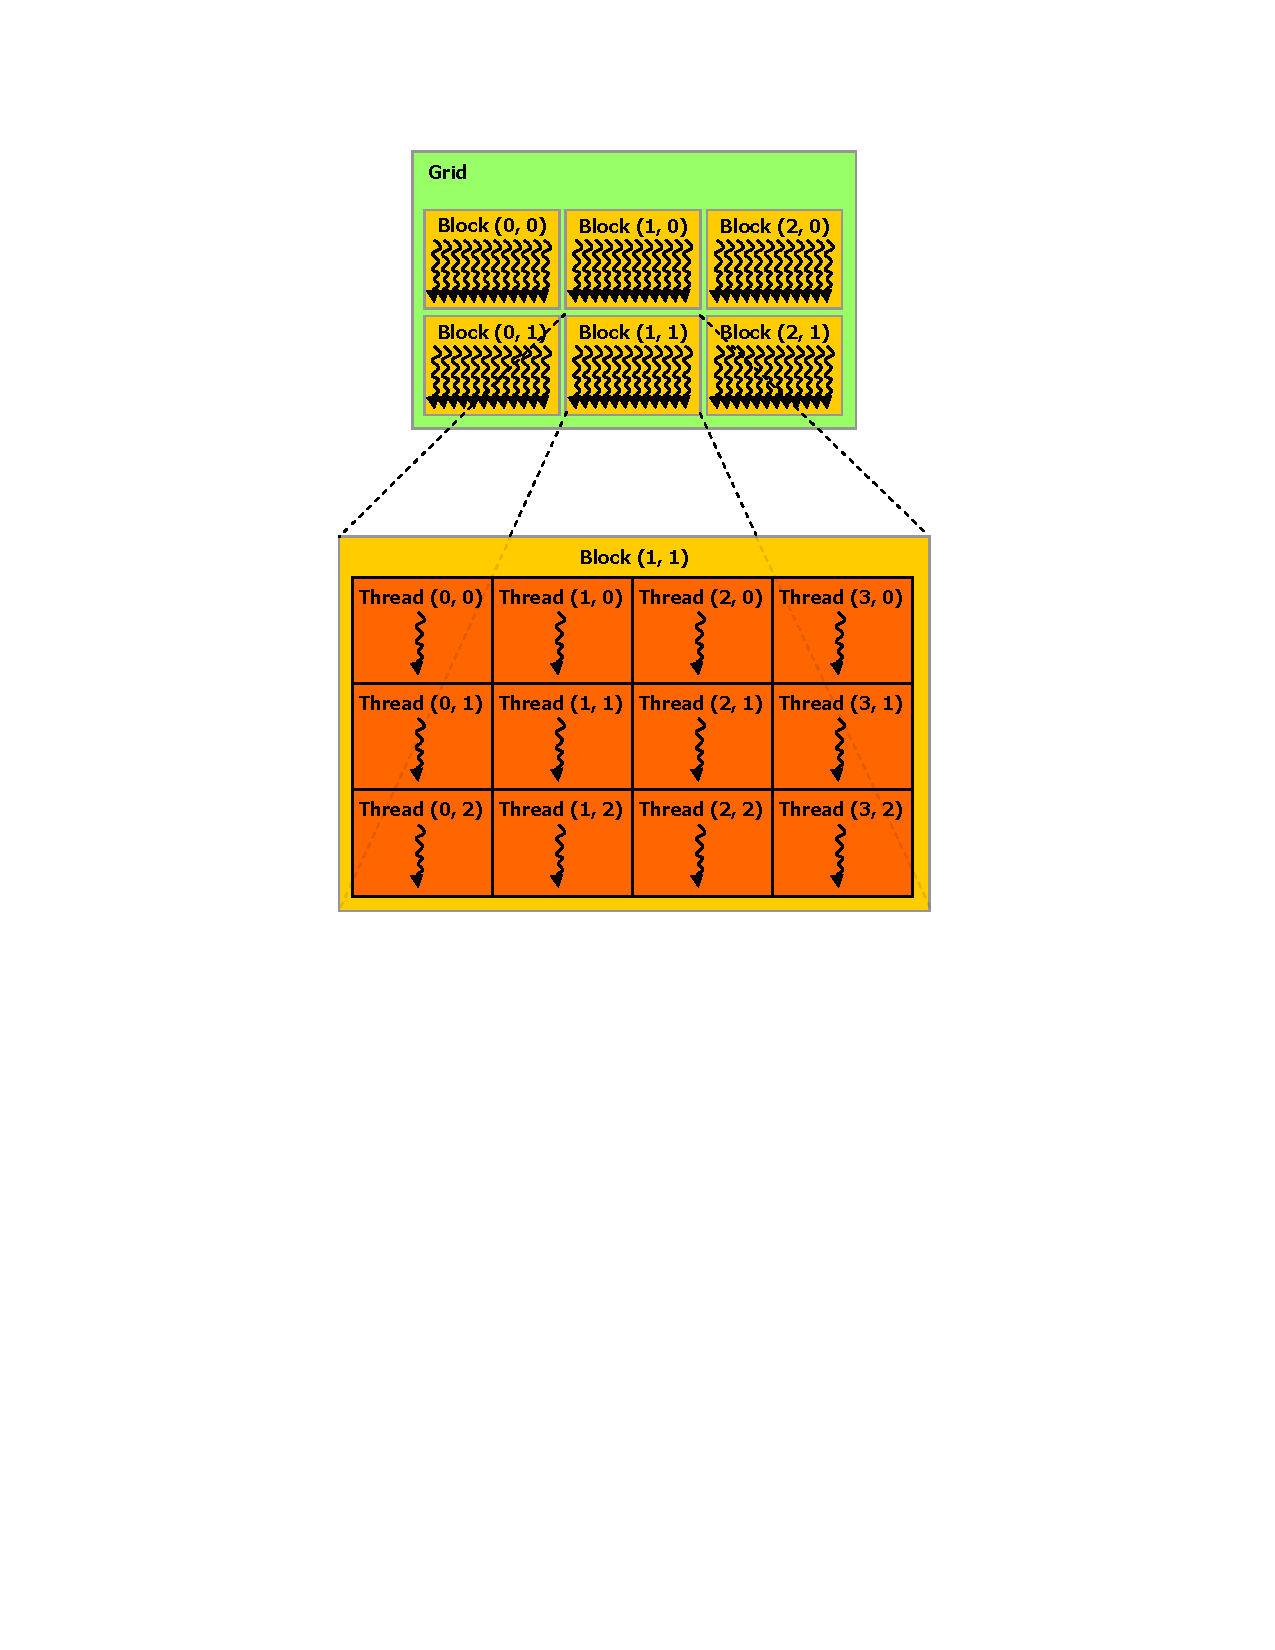
\includegraphics{figGridOfThreadBlocks.pdf}} 
    \renewcommand{\thefigure}{\thechapter.\arabic{figure}}
    \caption[GPGPU Thread Hierarchy]{\emph{}}
    \label{fig:grid_of_thread_blocks} 
\end{figure}

\subsubsection{Memory Model}










\section{KD-Tree Construction Using GPU}
In Chapter 3, we have defined a fast kd-tree construction algorithm \ref{algo:FindBestPlaneON} that has time complexity of \mycomplexitynlogn. Provided with a powerful modern GPU, it would be fascinating to optimize the algorithm for GPU to fully exploit the fine-grained parallelism of modern GPU architecture. 

%\refs:
% nvidia cuda programming guide

\subsection{Introduction}

In designing a kd-tree algorithm for the GPUs, how to maximally exploit the GPU's streaming architecture to parallelize the kd-tree construction. As discussed in the previous section, the massive parallel architecture of GPU requires \(10^{3}\) to \(10^{4}\) threads for optimal performance \cite{}<++>. The traditional optimized kd-tree construction algorithm adopt DFS (Depth-First Search) scheme to build a kd-tree, while CPU-based parallelized algorithm resort to DFS when the building process reaches a certain level. However, DFS order is not feasible when the algorithm comes to GPU, since the coherency of memory access is critical to GPU. BFS (Breadth-First Order) is an intuitive alternative approach, indeed BFS algorithm is much more suitable to take advantage of the GPU's architecture. Instead of finding split plane for each node greedily, by following BFS order the tree will be built level by level, every node at the same tree level spawns a new thread and the total number of threads doubles from the preceding step. This approach can fully exploit the massive data parallelism of GPU.

Memory management has always been a critical factor that has huge impact on the performance and feasibility of the both CPU and GPU kd-tree constructor. Dynamically allocating memory for kd-tree nodes and their AABBs as the building process goes will hurt the performance greatly making the algorithm unacceptably slow, this is mainly due to the overhead of memory management API on both CPU and GPU. This overhead can be reduced by pre-allocating a chunk of memory that is big enough to hold all the data dynamically created in the kd-tree construction. However, on the other hand, this lead to higher memory requirements as the scene complexity grows and potential memory wastage. More sophisticated memory scheme will be required. The memory management issue will be discussed later in the following chapter.

Another issue is the efficiency of the calculation of the node split costs. The previously described SAH method is important for maintaining the quality of kd-tree. However, precisely evaluating the costs of all the kd-tree nodes is too expensive for real-time applications. Therefore, vary recent approaches sacrificed SAH evaluations picking the median split instead until a certain level reached. Since the as the building process continues, the number of the triangles contained in a voxel of kd-tree node becomes smaller, leading less expensive SAH evaluation iterating over all the triangles. Therefore the number of triangles in an AABB is used as a threshold and it will be specified by the user. 

\subsection{Algorithm Description}
In this section, the GPU-based SAH kd-tree building algorithm will be presented. This algorithm follows the essential scheme as the construction algorithms previous described, it is a greedy, top-down manner as described in the following algorithm. 

\SetAlFnt{\small}
\begin{algorithm}[H]

        \SetKwFunction{buildKDTreeGPU}      {buildKDTreeGPU}
        \SetKwFunction{processLargeNodes}   {processLargeNodes}
        \SetKwFunction{processSmallNodes}   {processSmallNodes}
        \SetKwFunction{outputTreeNodes}     {outputTreeNodes} 

        \myfunc \buildKDTreeGPU{\mytriangles} \newline
        \Begin{
        \tcp{initialization stage}
        \emph{new} treeNodesList 

        \emph{new} workNodesList  
        \emph{new} smallNodesList
        \emph{new} nextNodesList    

        Create rootNode
        workNodesList.add(rootnode)

        \ForEach {\mytriangle\ \(\in\) \mytriangles} \bf in parallel
        {
        Calculate AABB for triangle \mytriangle
        }

        \tcp{process large node}
        \While{workNodesList is not empty} 
        {
        append workNodesList to treeNodesList
        clear nextNodesList
        \processLargeNodes{workNodesList, smallNodesList, nextNodesList}
        Swap nextNodesList and workNodesList
        }

        \tcp{process small node}
        \processSmallNodes{smallNodesList}
        workNodesList \leftarrow\ smallNodesList
        \While{workNodesList is not empty} 
        {
        append workNodesList to treeNodesList
        clear nextNodesList
        \processSmallNodes{workNodesList,nextNodesList}
        Swap nextNodesList and workNodesList
        }

        \tcp{output the kd-tree nodes}
        \outputTreeNodes{treeNodesList}
        }

        \caption{The \mynaive\ algorithm of finding the best SAH split plane}
        \label{algo:BuildKDTreeGPU} 
\end{algorithm}



\SetAlFnt{\small}
\begin{algorithm}[H]
    \SetKwFunction{processLargeNodes}       {processLargeNodes}
    \myfunc \processLargeNodes{ { {\bf in} workNodesList, {\bf out} smallNodesList, {\bf out} nextNodesList} 
    \Begin {
        \tcp{first step: group triangles into chunks}
        \ForEach{node \mynod\ in workNodesList \bf in parallel}
        {
            Group all triangles in \mynode into fixed size chunks
            Store the chunks in trianglesChunkList
        }

        \tcp{second step: compute per-node AABB}
        \ForEach{chunk \mytrichunk\  in trianglesChunkList \bf in parallel} 
        {
            Calculate the AABB of all triangles in \mytrichunk\ using standard reduction
        }
        Perform segmented reduction on per-chunk reduction result to compute per-node AABB

        \tcp{third step: split large nodes}
        \ForEach{node \mynode\ in workNodesList \bf in parallel}
        {
            \ForEach{side \myaabbside\ of the AABB of node \mynode\ }
            {
                \If{\mynode\ contains empty space larger than a threshold on side \myabbside}
                {
                    Cut off the empty space of \mynode\ on side \myaabbside\ 
                }
            }
            Split node \mynode at spatial median of the longest axis. 
            Two new child nodes are created.
            \ForEach{newly created child node \mynode\ }
            {
                add \mynode to nextNodesList
            }
        }

        \tcp{forth step: classify the triangles into child nodes}
        \ForEach{triangles chunk \mytrichunk\ in trianglesChunkList \bf in parallel}
        {
            \mynode \leftarrow the index of the node the chunk \mytrichunk belongs to
            \ForEach{triangle \mytriangle\ in \mytrichunk\ \bf in parallel} 
            {
                \If{\mytriangle\ intersects both child nodes of \mynode\ }
                {
                    \mylefttrilist\  \leftarrow \mytriangle
                    \myrighttrilist\ \leftarrow \mytriangle
                }
                Classify \mylefttrilist\ and \myrighttrilist\ into two child nodes.

                \Else {
                    Classify \mytriangle into the child node contains it    
                }
            }
        }

        \tcp{count triangles for child nodes}
        \ForEach{chunk \mytrichunk\ in the trianglesChunkList \bf in parallel}
        {
            \mynode \leftarrow the index of the node the chunk \mytrichunk belongs to
            Count triangles in the child nodes of \mynode.
        }

        \tcp{small node filtering}
        \ForEach{child nodes \mynode\ in nextNodesList \bf in parallel}
        {
            \If{\mynode\ is small node}
            {
                Add \mynode\ to smallNodesList
                Delete \mynode from nextNodesList
            }
    }
    \label{algo:ProcessLargeNodes}
\end{algorithm}

\SetAlFnt{\small}
\begin{algorithm}[H]
    \SetKwFunction{ProcessSmallNodes}           {ProcessSmallNodes} 

    \myfunc \ProcessSmallNodes{ {\bf in} workNodesList, {\bf out} nextNodesList }
    }

\end{algorithm}





%-------------------------

%-------------------------
% Chapter 5: Implementation and Result 
\chapter{Implementation and Results}
\setcounter{figure}{1}      % reset the figure counter
\label{ch:implementation_and_results} 



%-------------------------

%-------------------------
% Chapter 6: Conclusion
\chapter{Conclusion}  
\setcounter{figure}{1}      % reset the figure counter
\label{ch:conclusion} 



%-------------------------

%-------------------------
% Appendix 
\include{appendix}
%-------------------------

%\bibliography{C:/Users/lenovo/thesis/working/thesis/bib/refdb}  			%place your .bib files here
\bibliographystyle{ieeetr}               %the bibliography style to use
\bibliography{refdb}

\end{document}

